\documentclass[12pt,a4paper,oneside]{report}
%Vinayak Shankarrao Deolankar
\renewcommand{\baselinestretch}{1.5}
%---------------spacing between number and caption in lof-------------------- 
\makeatletter
     \renewcommand*\l@figure{\@dottedtocline{1}{1em}{3em}}
\makeatother
%------------Required Packages------------------------------------------------
\usepackage[english]{babel}
\addto{\captionsenglish}{\renewcommand{\bibname}{References}}
%-------------Multirow and multocolomn table-----------------------------------
\usepackage{multirow}
%---------------COLOR----------------------------------------------------------
\usepackage[dvipsnames]{xcolor}
\definecolor{ured}{HTML}{C00000}
\definecolor{ublue}{HTML}{0000FF}
%-----------------section numbering--------------------------------------------
%\setcounter{tocdepth}{3}
%\setcounter{secnumdepth}{3}
%------------------------------------------------------------------------------
\usepackage{cite}
%\usepackage{tcolorbox}
%------------------Math font and symbols---------------------------------------
\usepackage{amsmath}
\usepackage{amsfonts}
\usepackage{amssymb}
%-----------------------Theroum definition lemma--------------------------------
\usepackage{amsthm}
\theoremstyle{definition}
\newtheorem{definition}{Definition}[section]
\newtheorem{corollary}{Corollary}
%-------------------------Add figures-------------------------------------------
\usepackage{graphicx}
\graphicspath{ {images/} }
%-------------------------table------------------------------------------------
\usepackage{booktabs}
\usepackage{threeparttable}
\usepackage{float}
%------------------------------------------------------------------------------
\usepackage{array}
\usepackage[hidelinks]{hyperref}
\hypersetup{linktoc=all,}

\usepackage[left=1.5in,right=1in,top=1in,bottom=1in]{geometry}

%-----------------------Nomenclature Setting------------------------------------
\usepackage{nomencl}
\nomlabelwidth=3cm 
\makenomenclature
\renewcommand{\nomname}{Abbreviations}
%--------------------------Contents Name----------------------------------------
\addto\captionsenglish{\renewcommand{\contentsname}{INTENT}}
%---------------------for removing hyperindentation-----------------------------
\brokenpenalty=10000
\hyphenpenalty=10000
%-----------------------numbered discription------------------------------------
\usepackage{enumitem}
\newcounter{descriptcount}
\renewcommand*\thedescriptcount{\arabic{descriptcount}}
%------------------------figure numbering---------------------------------------
\usepackage{chngcntr}
\counterwithin{figure}{section}
\counterwithin{table}{section}
%\renewcommand{\thefigure}{\arabic{chapter}.\arabic{section}.\arabic{figure}}
%\renewcommand{\thetable}{\arabic{chapter}.\arabic{section}.\arabic{table}}
%-------------------------Indent to zero-------------------------------------
\setlength{\parindent}{0pt}
%------------------------landscape package-------------------------------------
\usepackage{pdflscape}
%\begin{landscape}
%\end{landscape
%---------------------------rotate figure--------------------------------------
\usepackage{rotating}
%\begin{sidewaysfigure}
%\end{sidewaysfigure}

%\begin{figure} 
%   \centering 
%   \begin{turn}{90}
%   \includegraphics[scale=0.60]{333.png}
%   \end{turn}
%   \caption{ MSCI Sector performances.} 
%   \label{Fig:16} 
%\end{figure}

%\begin{sidewaysfigure}} 
%   \centering 
%   \includegraphics[width=\textwidth]{TimeDefinitionsduringCloseOpenCycleforCBwithout} 
%   \caption{Time Definitions during Close-Open Cycle for CB without Switching Resistors}
%   \label{Fig:Time Definitions during Close-Open Cycle for CB without Switching Resistors} 
%\end{sidewaysfigure}

%\begin{sidewaystable}
%    \centering
%    \caption{Your caption here}
%   \begin{tabular}{ll}
%    First First & First Second\\
%    Second First & Second Second
%    \end{tabular}
%\end{sidewaystable}
%------------Fancy Header Setting-------------------
\usepackage{fancyhdr}
\lhead{}
\chead{}
\rhead{\thepage}
\lfoot{}
\cfoot{}
\rfoot{}
\renewcommand{\headrulewidth}{0pt}
\renewcommand{\footrulewidth}{0pt}
%--------------------------text subscript--------------------------------------
\usepackage{fixltx2e}

\usepackage{caption} 
\usepackage{subcaption}
\usepackage{ragged2e}
%------------------------------- et al ----------------------------------------
\usepackage{filecontents}
%-------------------------------Degree Symbol----------------------------------
\usepackage{siunitx}
\usepackage{textcomp}
%--------------------------------Roman enumerate---------------------------------
\usepackage{enumitem}
%---------------------------------Wrap Figure-----------------------------------
%\usepackage{wrapfig}
%--------------------------------Author and Title-------------------------------
\author{Vinayak Shankarrao Deolankar}
\title{Partial Discharge Analysis in Oil Filled Current Transformers 145 kV up to 3000 A}
%--------------------------------Custom biblography------------------------------

% Define the IEEE citation control command (not necessary if using IEEEtran class)
\makeatletter
\def\bstctlcite{\@ifnextchar[{\@bstctlcite}{\@bstctlcite[@auxout]}}
\def\@bstctlcite[#1]#2{\@bsphack
  \@for\@citeb:=#2\do{%
    \edef\@citeb{\expandafter\@firstofone\@citeb}%
    \if@filesw\immediate\write\csname #1\endcsname{\string\citation{\@citeb}}\fi}%
  \@esphack}
\makeatother
%---------------------------------------------------------------------------------


\begin{document}
\bstctlcite{IEEEexample:BSTcontrol}
%\nocite{*} %For print biblography
\pagenumbering{gobble}

\begin{titlepage}
%-----------------------FRONT PAGE------------------------------------------------
\begin{center}
~\\
\textit{\small The Thesis Entitled}\\
\vspace{1cm}
\textcolor{ured}{\textbf{\large PARTIAL DISCHARGE ANALYSIS IN OIL FILLED CURRENT TRANSFORMERS 145 kV up to 3000 A}}\\
\vspace{0.5cm}

\includegraphics[width=.30\textwidth]{universityLOGO}\\
\vspace{0.6cm}
\textit{\normalsize Submitted to}\\
\vspace{0.5cm}
\textcolor{ublue}{\textbf{\large Dr. BABASAHEB AMBEDKAR MARATHWADA UNVIERSITY, AURANGABAD}}\\
\vspace{1cm}
\textit{\normalsize In partial fulfilment of the Requirement for the Award of the Degree of}\\
\textbf{\large DOCTOR OF PHILOSOPHY}\\
\textit{\normalsize in}\\
\textbf{\normalsize ELECTRICAL ENGINEERING}\\
\textbf{\textit{\small By}}\\
\textcolor{ured}{\textbf{\normalsize Vinayak Shankarrao Deolankar}}\\
\textit{\normalsize Under the Guidance of}\\
\textcolor{ured}{\textbf{\large Dr. W. Z. Gandhare}}\\
\vspace{1cm}
\textbf{\normalsize FACULTY OF ELECTRICAL ENGINEERING}\\
\textbf{\large Dr. BABASAHEB AMBEDKAR MARATHWADA UNVIERSITY, AURANGABAD-431 004 (MS), INDIA\\
OCTOBER - 2017}
\end{center}
\clearpage
%-------------------------SECOND PAGE------------------------------------------------------
~\\
\textcolor{ured}{\textbf{\textit{\large PARTIAL DISCHARGE ANALYSIS IN OIL FILLED\\CURRENT TRANSFORMERS 145 kV up to 3000 A}}}
\vspace{2cm}

\textcolor{ublue}{\textbf{\large Ph. D. Thesis}}\\
\textit{\normalsize in Electrical Engineering}\\
\vspace{2.5cm}


\textit{\small Author}\\
\textcolor{ured}{\textbf{\large Vinayak Shankarrao Deolankar}}\\
\small Research Scholar
\vspace{3cm}

\textit{\small Under the Guidance of}\\
\textcolor{ured}{\textbf{\large Dr. W. Z. Gandhare}}\\
\vspace{0.5cm}

\small Director, G. S. Moze College of Engineering, Pune\\
\small Research Guide in Electrical Engineering\\
\small Dr. Babasaheb Ambedkar Marathwada University\\
\small Aurangabad - 431 004 (MS) INDIA
\vspace{2cm}

\textbf{\textit{\large OCTOBER 2017}}
\clearpage
%-----------------------INSIDE COVER PAGE -----------------------------------------------------
\begin{center}
~\\
\textbf{\large PARTIAL DISCHARGE ANALYSIS IN OIL FILLED CURRENT TRANSFORMERS 145 kV up to 3000 A}\\
\vspace{0.5cm}

\includegraphics[width=.3\textwidth]{universityLOGO}\\
\vspace{0.8cm}
\textit{\normalsize Submitted to}\\
\textbf{\large Dr. BABASAHEB AMBEDKAR MARATHWADA UNVIERSITY, AURANGABAD}\\
\vspace{1cm}
\textit{\normalsize for the Degree of}\\
\textbf{\normalsize Doctor of Philosophy}\\
\textit{\normalsize in} \\
\textbf{\normalsize Electrical Engineering}\\
\textbf{\small By}\\
\textbf{\large Vinayak Shankarrao Deolankar}\\
\textit{\normalsize Under the Guidance of}\\
\textbf{\large Dr. W. Z. Gandhare}\\
\vspace{1cm}
\textbf{\large FACULTY OF ELECTRICAL ENGINEERING}\\
\textbf{\large Dr. BABASAHEB AMBEDKAR MARATHWADA UNVIERSITY, AURANGABAD-431 004 (MS), INDIA\\
OCTOBER - 2017}
\end{center}
\clearpage


%-----------------------CERTIFICATE-------------------------------------------------------------
\begin{center}
\large \textbf{Dr. Babasaheb Ambedkar Marathwada University\\
Aurangabad (M. S.) - 431 004}\\
\vspace{0.5cm}

\includegraphics[width=.3\textwidth]{universityLOGO}\\
\vspace{0.5cm}
%\addcontentsline{toc}{chapter}{\numberline{}Certificate}
\textbf{\large CERTIFICATE}\\
\end{center}
\normalsize This is to certify that the thesis entitled \textbf{\textquotedblleft Partial Discharge Analysis in Oil Filled Current Transformers 145 kV up to 3000 A\textquotedblright}, which is being submitted herewith for the award of the \textbf{\textquoteleft Degree of Doctor of Philosophy\textquoteright ~in \textquoteleft Electrical ~Engineering\textquoteright} of \textbf{~Dr. Babasaheb Ambedkar ~Marathwada University, Aurangabad}. This is the result of the Original Research Work and Contribution by \textbf{\textquoteleft Vinayak Shankarrao Deolankar\textquoteright} under my supervision and guidance at Government College of Engineering, Aurangabad. The work embodied in this thesis has not formed earlier for the basis of the award of any degree or compatible certificate or similar title of this for any other diploma/examining body or university to the best of knowledge and belief. 

\vspace{0.5cm}
Place: \textbf{Aurangabad}\\
Date~: \textbf{~~~/~~~/}\\

\hspace{2.2in}
\begin{minipage}{4in}
\vspace{0.5in}
\begin{center}
\textbf{Dr. W. Z. Gandhare}\\
Research Guide\\
Electrical Engineering\\
Faculty of Engineering \& Technology\\
Dr. Babasaheb Ambedkar Marathwada\\University, Aurangabad\\
\end{center}
\end{minipage}

\clearpage
%-----------------------ABSTRACT-------------------------------------------------------------
\chapter*{ABSTRACT}
%\addcontentsline{toc}{chapter}{\numberline{}Abstract}
This research study consist of effect of Partial Discharge on high voltage oil filled current transformers. As high voltage electrical equipments are under various stresses such as thermal, mechanical, insulation strength, electrical stress which will deteriorate the performance and reliability of instrument. Also the defects during the manufacturing process, design aspects, ageing effect, voids formed in insulating material oil or solid plays major role in effective functioning of substation in totality.

In this study different sizes of voids in the insulating material are considered. Voids forms the capacitance in the electrical circuit and will have the different electrical effects in the circuit. Capacitance for different void sizes are tabulated.

For study and analysis purpose the mathematical model for oil filled current transformers of 145 kV up to 3000 A and void in oil insulation were considered. Charge due to various capacitance, the effect of diameter, volume were studied and analysed for the effect on partial discharge. 

A Simulation models for 145 kV current transformer current up to 3000 A were used in MATLAB to study the effect of various sizes of voids during steady state operations. The waveform pulses shows the effects in amplitude, width, number of pulses in sine wave. The short circuit and transient has high impact on life and deterioration of high voltage equipments. Since the voltage level and current are very high, electrical stress are generated, surrounding weak sections also contributes which leads to the formation of partial discharge and its impact leads to the failure of equipments. Simulation also done for different sizes of voids in insulation considering short circuit and transient conditions. The waveform show dense pulses, high amplitude and effect of transients on waveform. Laboratory results were studied on current transformers 145 kV, 3000/1, 2400/1, 600/5, 200/1 ratios for accuracy limit factory, ratio error, phase error, instrument security factor, high voltage test results during normal operating condition i.e steady state and effect after transients or deterioration of insulating parameters of materials. The ratio error and phase error results were compared for steady state and transient conditions. 

\clearpage

%-----------------------DECLARATION-------------------------------------------------------------
\begin{center}
\large \textbf{Dr. Babasaheb Ambedkar Marathwada University\\
Aurangabad (M. S.) - 431 004}\\
\vspace{0.5cm}

\includegraphics[width=.3\textwidth]{universityLOGO}\\
\vspace{0.5cm}
%\addcontentsline{toc}{chapter}{\numberline{}Declaration}
\textbf{\large DECLARATION}\\
\end{center}

\normalsize I ~hereby ~declare ~that ~the ~work ~presented ~in ~the ~form ~of ~thesis ~entitled \textbf{\textquotedblleft PARTIAL DISCHARGE ANALYSIS IN OIL FILLED CURRENT TRANSFORMERS 145 kV up to 3000 A\textquotedblright} is an original research work carried out by me under the guidance of Dr. W. Z. Gandhare, Director, G. S. Moze College of Engineering, Pune, and has not been previously submitted to this or any other University for the award of degree, diploma, associate ship, or any other similar title.

\vspace{0.5cm}
Place: \textbf{Aurangabad}\\
Date~: \textbf{~~~/~~~/}\\

\hspace{2.2in}
\begin{minipage}{4in}
\vspace{0.5in}
\begin{center}
\textbf{Vinayak Shankarrao Deolankar}\\
Research Scholar
\end{center}

\end{minipage}
\clearpage

%%-----------------------EVALUATION CERTIFICATE-----------------------------------------------
%\begin{center}
%\large \textbf{Dr. Babasaheb Ambedkar Marathwada University\\
%Aurangabad (M. S.) - 431 004}\\
%\vspace{0.5cm}
%
\includegraphics[width=.3\textwidth]{universityLOGO}\\
%\vspace{0.5cm}
%
%\textbf{\large EVALUATION CERTIFICATE}\\
%\end{center}
%
%
%\normalsize \textbf{Mr. Vinayak Shankarrao Deolankar} has done the appropriate work for the fulfilment for the award of \textquotedblleft Degree in Philosophy\textquotedblright ~in \textquoteleft Electrical Engineering\textquoteright ~of Dr. Babasaheb Ambedkar Marathwada University, Aurangabad (M.S.).
%
%\hspace{1cm}
%\begin{minipage}{4in}
%\vspace{0.5in}
%1.~Chairman:\\
%\\
%2.~External Referee:\\
%\\
%3.~Guide:\\
%\\
%Place: \textbf{Aurangabad}\\
%Date~: \textbf{~~~/~~~/}\\
%\end{minipage}
%
%\clearpage



\tableofcontents
\clearpage

\pagenumbering{roman}

\listoffigures
\addtocontents{lof}{\protect\addcontentsline{toc}{chapter}{\numberline{}List of Figures}}

\listoftables
\addcontentsline{toc}{chapter}{\numberline{}List of Tables}

\printnomenclature
\addcontentsline{toc}{chapter}{\numberline{}Abbreviations}
\end{titlepage}
%\pagestyle{fancy}

\nomenclature{CT}{Current Transformer}
\nomenclature{PD}{Partial Discharge}
\nomenclature{pC}{Pico Coulomb}
\nomenclature{C}{Capacitance}
\nomenclature{e\textsubscript{r}}{Relative Permittivity}
\nomenclature{SIWL}{Switching Impulse Withstand Level}
\nomenclature{IFS}{Instrument Security Factor}
\nomenclature{ALF}{Accuracy Limit Factor}
\nomenclature{BIL}{Basic Insulation Level}
\nomenclature{VLF}{Very Low Frequency testing}
\nomenclature{Bur}{Burdon} % List of Abbrivations

\chapter{INTRODUCTION}
\pagestyle{fancy}
\thispagestyle{empty}
\pagenumbering{arabic}
%Introduction

\section{Introduction}
\justify The High voltage electrical instruments have a unique problem of failure due to the breakdown of insulation strength. As the insulation of live electrical conductor fails, the purpose and function of electrical instrument stop leading toward the failure of the system. Because of partial discharge of Current Transformers will give rise to the failure of product resulting in the disruption in the supply of the system. Measurement of Partial discharge will help in predicting failure of insulation strength of Current Transformers, and corrective actions can be planned to avoid the failure of Instrument. Current transformers are used for measurement and protection application. The current transformers in electrical system step down the primary current to 5 A or 1 A. \setlength{\parskip}{1em}

Current ~Transformers ~are ~designed ~considering ~accuracy ~and ~protection requirements and current carrying capacity of the system, best insulating materials, cores and other materials are used \setlength{\parskip}{0em} \cite{crichton1989partial}.

\subsection{Partial discharge phenomenon}
Partial discharges are discharges of electrical energy in insulation material in high voltage electrical equipment's in the form small sparks. Electrical breakdown occurs after failure of insulation material due to partial discharge effect. The capacity and capability of insulation media and analysis of Partial discharge help in knowing insulation strength of instrument. The partial discharge of high voltage electrical instruments can be measured off line or Online. Measurements of partial discharge help in knowing healthy status of instruments current transformers. The electric dielectric strength and tensile strength of material decide the capability of current flow and electrical discharge during operating conditions. The insulating materials used in high voltage instruments are oil, SF\textsubscript{6} gas or mica and for low voltages epoxy, polyesters are used as insulating material. The breakdown current in the system can be known by measuring partial discharge \cite{van1994physics, danikas1998some, paithankar1997can}.\setlength{\parskip}{1em}

High voltage electrical equipment undergoes various kind of stresses during operating conditions. The electrical conducting material has thermal, chemical, mechanical stress. The reliability of electrical instrument depends upon susceptibility to these stress.

The partial discharge will cause stresses, and it will make insulation strength of oil, insulating material used in a conductive winding. The weakening or failure of insulating material will lead to generate small voids in the instrument. This will initiate the process of partial discharge and will lead to failure of an instrument. Partial discharge gives the indication of instrument failure and warning of instrument breakdown. The electric arc formed in partial discharge will reduce the dielectric strength of the material and will also have an effect on mechanical properties. The insulation of winding will become weak, and hence there will be breakdown and possibility of a fault in the system. Partial discharges in a current transformer give the indication futuristic failure. Thus, partial discharge is the tool to identify insulating strength of Current transformers \setlength{\parskip}{0em} \cite{kolev1998partial}.

\subsubsection{Partial discharge phenomenon in high voltage current transformers}
The conductive live part of electrical instruments is protected by insulation strength of the material used. The insulation failure is due to either aging effect of insulation or failure of dielectric strength of the material. If we know the reasons of insulation failure, the corrective action will have improvement and avoid re occurrence of a failure.\setlength{\parskip}{1em}

The main application of current transformers is protection through relays or for measurement through meters.

The application of Current Transformers is to maintain accuracy in measurements and can be achieved by controlling manufacturing processes and best quality of raw material. The measurement of Partial Discharge helps in knowing the potential reasons for equipment failure \cite{ren2006simulation}.

The electrical stresses in the insulation of high voltages current transformers give discharges of energy. This phenomenon is called partial discharge which will discharge energy continuously but will not lead to the failure of equipment. If this discharge is continued with high strength will lead to weaken insulation strength. The electrical stress increases, after certain limit it will lead to complete failure of the instrument. The existence of voids in solid or liquid insulating media will also reduce the insulating strength of dielectric media. This partial discharge phenomenon can occur in this void. When the electrical stresses in the void are more, will lead to breakdown and discharge phenomenon will occur \cite{kolev1999approach}.

Partial discharge is defined as electric charge Coulomb C. Since this charge is very minor defined in terms of pico. Unit of partial discharge is pico coulombs pC.

The partial discharge can be controlled by major actions during the manufacturing process in controlled environmental conditions. Avoid the voids in paper and oil insulating material. Use of a quality insulating material having high dielectric insulation \setlength{\parskip}{0em}\cite{satish1994artificial}.

\begin{figure}[h!]
    \centering
    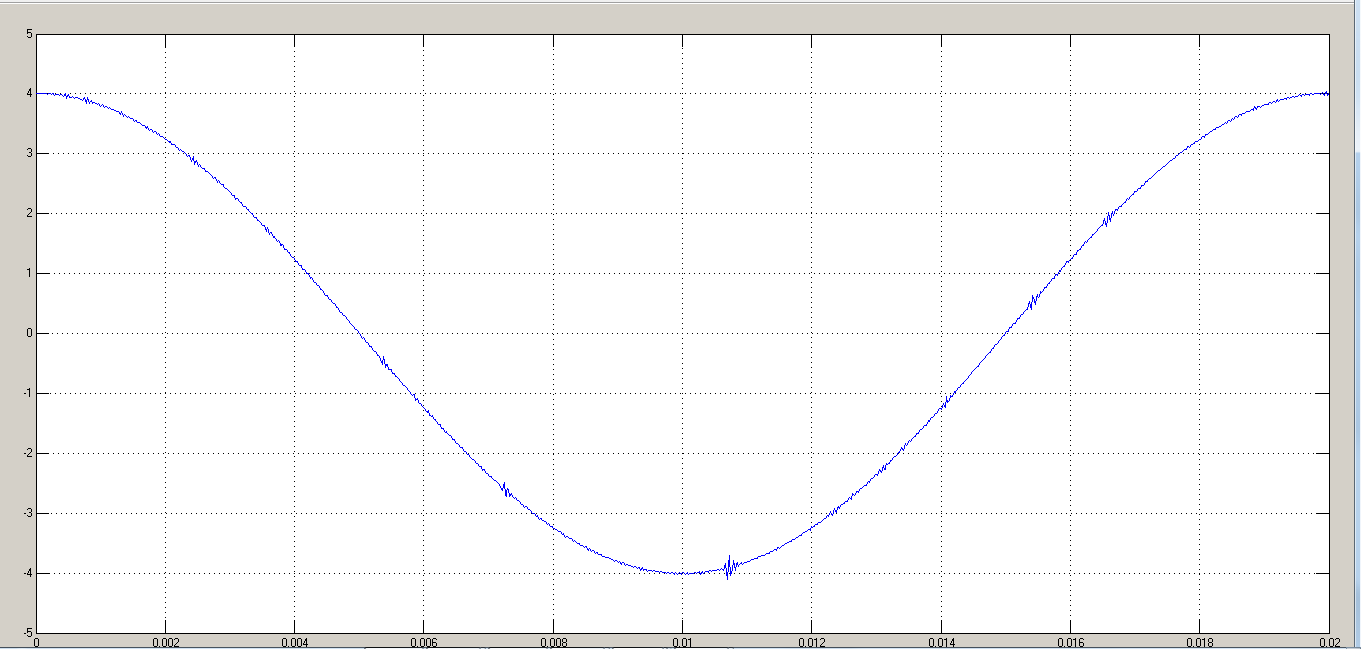
\includegraphics[width=\textwidth]{InputACSineWave145kV}
    \caption{Input AC Sine Wave 145 kV}
    \label{fig:Input AC Sine Wave 145 kV}
\end{figure}

\begin{figure}[h!]
    \centering
    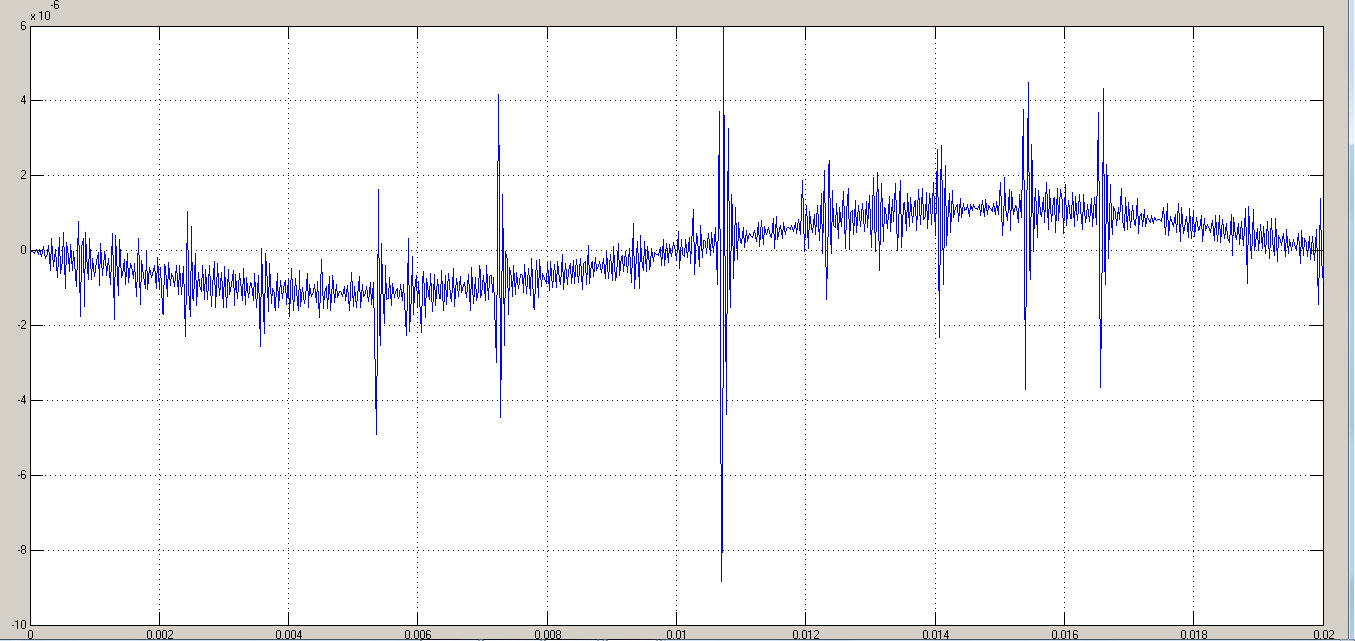
\includegraphics[width=\textwidth]{OutputACSineWave145kVwithPartialDischargepulses}
    \caption{Output AC Sine Wave 145 kV with Partial Discharge Pulses}
    \label{fig:Output AC Sine Wave 145 kV with Partial Discharge Pulses}
\end{figure}

\begin{figure}[h!]
    \centering
    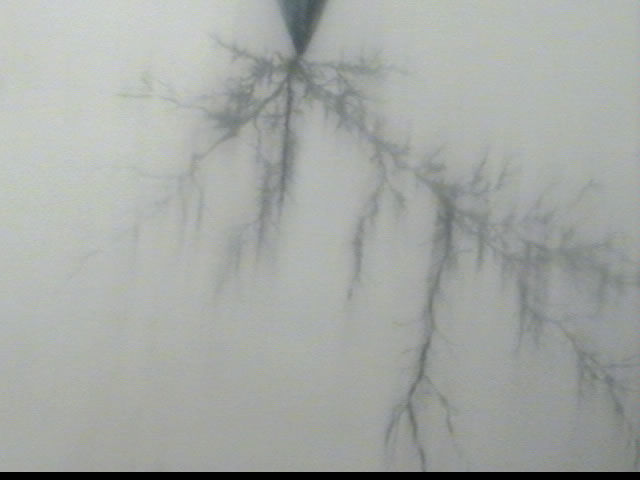
\includegraphics[width=\textwidth]{TreeingProcessduetoPartialDischarge}
    \caption{Treeing Process  due to Partial Discharge}
    \label{fig:Treeing Process  due to Partial Discharge}
\end{figure}

\begin{figure}[h!]
    \centering
    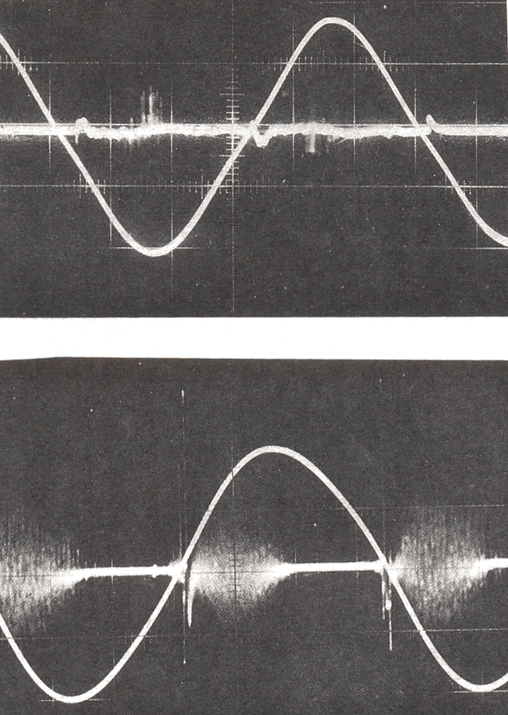
\includegraphics[width=\textwidth]{PartialDischargeWaveformDue}
    \caption{Partial Discharge Waveform Due to Voids in Insulating Material}
    \label{fig:Partial Discharge Waveform Due to Voids in Insulating Material}
\end{figure}

\clearpage 
Effect of Partial Discharge on Current Transformer
\begin{enumerate}


\item The phenomenon of partial discharge in high voltage current transformers will lead to the complete breakdown in the electrical network. The operation and performance will be deteriorated.

\item For study and analysis of partial discharge in current transformers, a Simulink model took for reference and effect due to partial discharges studied. The voids and insulation strength decided the partial discharge in oil filled current transformers. Also, the voltage level of current transformers will contribute to partial discharge.

\item From the Simulink model, different sizes of voids partial discharge pulses are studied and a number of PDs, magnitude, the frequency is calculated. This helps in knowing PD trend and further this data can be utilized to know the strength of insulation in high voltage current transformers.

\item The PD waveforms from Simulink model and calculated parameters used for oil and insulation papers sample, the characteristic of PDs has been studied.

\item The continuous Partial discharge in current transformers will reduce the insulation strength and will form the breakdown of electrical stress in the long term.

\item Partial discharge process leads to reduce insulation strength of insulating media oil and paper and will permanently damage the quality of insulation.

\item Partial discharge measurements are done to study effects caused due to PDs on insulation oil and can help in knowing the life of current transformers or actions for preventive maintenance \cite{gutfleisch1995measurement, bartnikas2002partial, karmakar2009partial}.

\end{enumerate}

\pagebreak 
\section{Motivation}
Detection and measure Partial Discharge Phenomenon in High Voltage Current Transformers ~145kV ~which ~is ~the ~main source ~of ~failure. The ~effect on the performance of insulation used in High Voltage Current Transformers 145kV during working conditions over the period of time with high stress needs to be studied in various conditions.\setlength{\parskip}{1em}

High voltage electrical instruments always have the problem of insulation failure because of insulation deterioration over the period of time. When the insulation fails, the electrical instrument gets damaged to the nonrecoverable status. Hence the study of Partial discharge in high voltage current transformers will help in understanding effects on insulations medium, preventive maintenance planning and healthy life of instruments. 

Application of High Voltage Current transformers is for measurement as CTPT unit and protection supply to relays in the circuit. The purpose of the current transformer is to step down current in the system to 5A or 1A which is measurable value \cite{karmakar2009monitoring}.

A current transformer is instrument transformer which reduces secondary current with reference to the ratios to the primary current. Thus it defined in terms of the ratio of primary to secondary current. As these transformers are used for measurement purpose accuracy is most important.

The variable flux in toroidal cores decides the current in the secondary of the current transformer. The secondary of the current transformer is defined in terms of turn ratio. The primary ampere turns helps in magnetizing the core and secondary current is induced \cite{kuffel2000high, kreuger1989partial, naiduhigh }.

The current transformers are designed considering current flowing in the primary circuit, accuracy, and ratios required, material of insulation and cargo material of cores.\\

Partial Discharge in High voltage Current Transformers is resulting in the breakdown of Instrument. A study needs to be done for analysis, reasons, and actions during the manufacturing process. Based on study improvements will be suggested to improve the performance of Product in Service. The breakdown will damage not only the Current transformer but also nearby Instruments in Sub Station. Hence study is required on Partial Discharges of Current Transformers which are going High Electrical Stress in working condition. The study is required for testing of Current Transformers  \cite{Proceedingsof2008International}.

During the manufacturing process, current transformers undergo various type test and routine test to meet the specifications at national and international level.

Some of the routine tests conducted on current transformers are\setlength{\parskip}{0em} 

\begin{enumerate}[label=\Roman*.]
\item Comparison test with standard CT, \textit{i.e.}, accuracy and phase error as per standard specifications

\item Insulation breakdown to know the strength of insulation by applying the high voltage to winding

\item Effect of temperature on the performance of insulation

\item Tan delta and insulation breakdown of oil

\item Short circuit current flowing capacity of insulating material
\end{enumerate}

\pagebreak 
\section{Objectives}
The objectives of this research work are to:
\begin{enumerate}
\item Propose Manufacturing Industries for Improvement in Performance of High Voltage Current Transformers

\item Study, Analyze and Measure Premature Failure of High Voltage Current Transformers

\item Provide actions in Manufacturing processes to minimize Partial Discharge phenomenon

\item Study On line and Off line Testing of Partial Discharge in High Voltage Current Transformers

\item Develop Mathematical Modeling of High Voltage Current Transformers

\item Simulate Model for High Voltage Current Transformers in Steady State Condition

\item Simulate Model for High Voltage Current Transformers in Short Circuit and Transient Condition
\end{enumerate}

\pagebreak 
\section{Theme}
The theme for this research work based on Partial Discharge Analysis of high voltage oil 
Filled current transformers 145 kV up to 3000 Amp used in high voltage Sub stations.
The study is concentrated on Improving the performance of Current Transformers hence
data from field and manufacturing process were conducted.\setlength{\parskip}{1em}
 
Having taken a due note of restraints upon efforts, resources and time, the study is
Confined mainly two areas, effect on Current Transformers during steady state Conditions
and during Short Circuit and Transient condition. Using MATLAB / Simulink model used
for comparative Study and the performance analysis carried out on the basis of various void
sizes developed and worked for effect of various void sizes on performance of Current 
Transformers. On the basis of results obtained improvement in existing manufacturing
process were suggested\setlength{\parskip}{0em}.

\begin{figure}[h!]
    \centering
    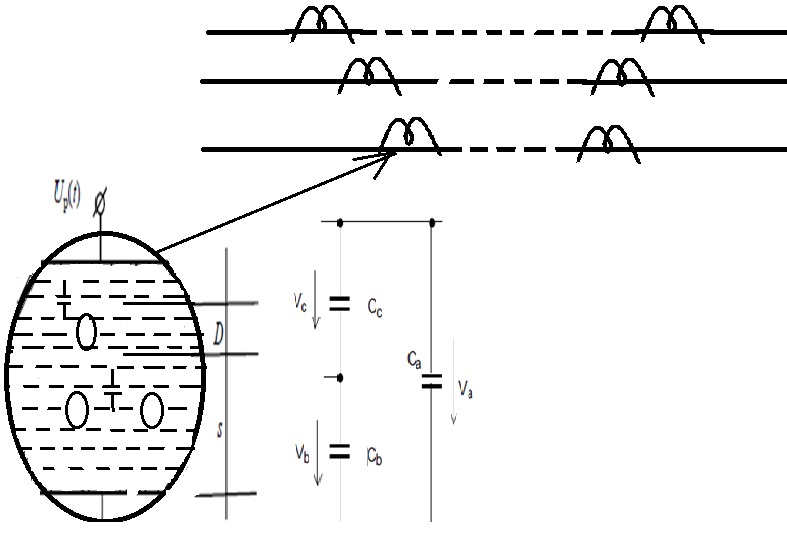
\includegraphics[width=\textwidth]{HighVoltageTransmissionLineWithCurrentTransformers}
    \caption{High Voltage Transmission Line With Current Transformers}
    \label{fig:High Voltage Transmission Line With Current Transformers}
\end{figure}

\pagebreak 
\section{Organization}
The ~research work titled \textquotedblleft Partial Discharge Analysis in High Voltage Filled Current Transformers 145 kV up to 3000 A\textquotedblright ~is organized in this Thesis among five chapters as per follow.\setlength{\parskip}{1em}

The first chapter gives Introduction of partial discharge phenomenon, and its effects on high voltage oil filled current transformers were given. The need and motivation for this research work mentioned and Objectives of this study work described. The Theme of the complete study work is presented.

A summary of the exhaustive literature survey is represented in second chapter. An overview of partial discharge and its effect on the performance of high Voltage electrical instruments in particular, oil filled current transformers were discussed in details.

Work done on System Development were discussed in third chapter. With the help of mathematical model of current Transformer and using MATLAB/SIMULINK software representing the steady state and Short circuit and transient conditions were run ~for different void sizes. Having taken ~various data ~from field ~and manufacturing process, need for developing Simulink model evolved to see the PD effect During Steady state, Short Circuit, and Transient Conditions. To attain Objectives of the study Manufacturing process of High Voltage Current Transformers were studied. Process Parameters, Insulation material, and strength, testing procedures, detection of Partial Discharge were studied. Analysis of these data was done and studied to meet Objectives. 

The Performance Analysis for the Simulink model mentioned in chapter 3 was done and explained in fourth chapter. Based on Collected data PD measurement were converted and Simulink model developed. The performance needs to be analyzed during steady state, Short Circuit and transients hence two Simulink models were developed. Data and PD were simulated with various kV applied and performance was interpreted and analyzed in the form of wave forms, strength and magnitude of partial discharge, number of partial discharges and its frequency of occurrence. PD pulses were observed for evaluation for different kV. This data was interpreted to find root causes of failures and problems to eliminate defects and effective corrective actions.

In the fifth chapter conclusion of the research work, future scope and the application of this research work are mentioned. 

To attain the above objectives and for getting information on Partial Discharge during ~Online ~performance of Current ~Transformers for ~145 kV ~survey ~was conducted of various Sub stations of 145 kV. Data of Various faults, failures, and analysis were conducted to get First-hand information on finding various information and to find reasons for Partial discharges.

As these High voltage current transformers and its electrical insulation undergo Various Thermal Stress, Chemical Attack and Abrasion due to excessive heat. From this model, PD Effect is studied for various kV voltages and different void sizes. Data collected for the number of PD, Frequency, Amplitude and predicted for PD effect. 

To Study, analyze performance High Voltage Current Transformers in field 145 kV Substations were selected. The performance in the field monitored during various conditions. Data collected for on line failures, its causes, various Measurements and its correlation with the performance of Current Transformers.

To Study the manufacturing process of High Voltage Current Transformers and collected data of various parameters which may lead to failures in Field. The Manufacturing process parameters such as High Vacuum level, Temperature, Oil low rate, Quality of Insulation material was studied and data collected. Acceptable limit of PD is between 5 pC to 10 pC. The Interpretation of data to Improve performance of PD were suggested.\setlength{\parskip}{0em}

%\setlength{\parskip}{1em}
%
%
%
%\begin{figure}[h!]
%    \centering
%    \includegraphics[width=\textwidth]{}
%    \caption{}
%    \label{fig:}
%\end{figure}
%
%
%
%\begin{table}[h!]
%\begin{threeparttable}
%\renewcommand{\arraystretch}{1.3}
%\caption{Percentage of Maf Rate and Mif Rate per Failure Mode, Third Inquiry.}
%\label{table:Percentage of Maf Rate}
%\centering
%\small
%\begin{tabular}{| >{\arraybackslash}m{1.9in} |>{\centering\arraybackslash}m{0.6in} |>{\arraybackslash}m{3in} |}
%
%%\begin{tabular}{| l | c | l |}
%\hline
%\multicolumn{1}{|c|}{\textbf{MaF failure mode}}	&	\textbf{MaF(\%)}	& \multicolumn{1}{|c|}{\textbf{Comments}}								\\ \hline
%Does not close on command	&	28.2				& Mainly with live tank circuit breakers			\\ \hline
%Does not open on command	&	16.4				&													\\ \hline
%Closes without command		&	0.2					&													\\ \hline
%Opens without command		&	5.4					&													\\ \hline
%Fails to carry the current	&	1.3					&													\\ \hline
%Dielectric breakdown		&9.9					& Breakdown to earth: 5\%, Internal breakdown across open pole, during opening operation = does not break the current: 1.9\%, Other across open pole: 1.8\%, Breakdown between poles: 1.2\%					\\ \hline
%Locked in open or closed position & 25.1			& Alarm has been triggered by the control system	\\ \hline
%Loss of mechanical integrity&	8.1					& Mechanical damage of parts						\\ \hline
%Other						&	5.2					&													\\ \hline
%Total						&	100					&													\\ \hline \hline
%\multicolumn{1}{|c|}{\textbf{MiF failure mode}}	& \textbf{Mif(\%)}		& \multicolumn{1}{|c|}{\textbf{Comments}}									\\ \hline
%Air or hydraulic oil leakage&	20.3				& In operating mechanism							\\ \hline
%Small SF\textsubscript{6} gas leakage		& 35.6					& Large leakage will give MF-mode \textquotedblleft
%Locked\textquotedblright
%			\\ \hline
%Oil leakage in grading capacitors &	1.0				&													\\ \hline
%Change in functional characteristics& 28.4			& 6.8\% mechanical; 3.3\% electrical 18.3\% control%
%													  and auxiliary systems								\\ \hline
%Other and no answer			& 14.6					&													\\ \hline
%Total						& 100					&													\\ \hline
%\end{tabular}
%%\begin{tablenotes}
%%\item \cmark -- functionality is available. \hspace{0.5in} \xmark -- functionality is not available.
%%\end{tablenotes}
%\end{threeparttable}
%\end{table}
%
%
%\section{Motivation}
%
%
%\clearpage
%\section{Objectives}
%
%
%\clearpage
%\section{Theme}
%
%\setlength{\parskip}{0em}
%\clearpage
%\section{Organization} 
%
%\subsubsection*{Chapter 1}

\chapter{LITERATURE SURVEY}\label{chp:lit.survay}
%Literature Survey

\section{Overview of Partial Discharge}

\subsection{Partial discharge phenomenon}
Partial discharges are a symptom of deterioration of insulation of the current transformer winding. Thus, partial discharge testing helps in determining the maintenance requirements of such high voltage Current Transformers\setlength{\parskip}{1em}.

Partial Discharge testing can be done On line or Off line which indicates that partial discharges indeed do occur. The partial discharges may only occur for a short time before failure with some types of failure mechanisms To prevent in-service failures of Current Transformers, continuous monitoring is necessary. Inexpensive continuous partial discharge monitor is available. The partial discharge monitoring will only be cost-effective for very critical process for high voltage current Transformers where in-service failures may have large financial consequence

The confirmation of the occurrence of partial discharges depends on the experience of the maintenance staff. The partial discharges characteristics caused by failures can ~be ~distinguished ~by ~noises ~and ~evaluating ~the time, ~voltage ~and ~phase characteristics. The phase is useful in investigating characteristics \cite{kim2003acoustic}.

Research activities are carried out on partial discharges phenomenon in solid, liquid and gaseous insulating materials used in high voltage current Transformers. The input voltage to the Current Transformers plays a significant role on the partial discharges. Phase shift during discharge occurrence can relate with the role of the space charge around the discharge sites in solid and liquid materials. The effects of partial discharges in solid are different with partial discharges in the liquid material. The Partial discharge magnitude in solid as well as in liquid strongly depends on partially applied voltage. Partial discharge probability in solid is strongly dependent on the time derivative of the applied voltage, but discharge probability in the liquid is strongly affected by the instantaneous applied voltage \cite{chen2008partial, forssen2008partial, standard200060270}. 

Partial Discharge generates the signals which can be detected by acoustic sensors. Partial discharge sources in current transformers can be detected by using acoustic methods. For the acoustic method, the signals of constant velocity are detected by acoustic a sensor which gives feedback on insulation condition of the solid and liquid material. Sometimes when the velocities of signals are not constant and will detect the wrong location of partial discharge. The pulses generated by partial discharge phenomenon may deform before reaching to the sensors and will give wrong indications. The deformation of the pulse depends upon the medium of pulse and distance traveled by the pulse. Thus sensor signaling cannot be correct representation partial discharge. Thus incorrect signals will give wrong sensing and fault detection of partial discharge. The location of the source of partial discharge can be known from the frequency of input pulse detection by the sensor which helps in identifying location of partial discharge inside the instrument.

 The Partial discharge detection system in high voltage equipment contains an analysis of distribution. The discharge on the surface or internal insulation failure causes the weakening strength of insulation over the period and lead to total failure of insulation system to avoid the effect on the life of insulation it is necessary to measure the discharge and internal condition of an instrument \cite{kuffel2000high2}.
 
Now a day's transmission line voltage level has increased above 400 kV line to 765 kV, 1000 kV, 1200 kV due to rise in demand of electrical energy. The advantage of high voltage line, transmission line loss is reduced but requires very high level of insulation. 

When the field intensity level goes above a particular level in high voltage equipment, generation of nonuniform field causes weakening of solid, liquid or gaseous insulation. The discharge direction depends upon the energy level generated by the partial discharge phenomenon. The partial discharge analysis depends upon the magnitude of discharge, insulation weakening and voltage level \cite{gockenbach2004partial}

In our study, a high voltage current transformer 145 kV up to 3000 A is selected. A detailed description including technical details of the test set up, graphical analysis of PD distributions of the sample with observation table and conclusions obtained are mentioned.

The partial discharge analysis in solid insulation can be done by the electro-optical measurement system.

Partial discharge monitoring can be done Online to avoid failure of power equipment. Acoustic emission is suitable to measure online partial discharge. The effect of partial discharge on insulation depends upon the magnitude and strength of Partial discharges. The deterioration of insulation is different for partial discharge pulses. The acoustic emissions are detected by the sensors inside the instrument. The signals issued by sensors are given to oscilloscope connected to the computer. The amplitude of the signal is analyzed for frequency magnitude, median, band, and these parameters are used for knowing the level of partial discharges \cite{bengtsson1996status}.

The high voltage equipment is under electrical stress which discharges energy due to the internal dissipation of energy from the various insulating material, hence consideration is given during design to decide insulating parameters, material, the distance between live parts. The electronic equipment which operates at high switching frequencies produces a corona. The corona voltages at high frequency are lower than the breakdown voltage. The breakdown data can be obtained from 10 kHz to 30 kHz frequency \cite{naiduhigh2}.

In liquid insulation oil, the partial discharge looks as streamers. Due to electric stress in equipment, this discharge in the insulation affects the performance of insulation. The partial discharge in oil is always due to the nonuniform field.

 The partial discharges are defined as a charge in Coulomb q. Generally, the value of partial discharge is E-9 hence defined in pC and phase angle in degree. The partial discharge phenomenon takes place in both cycles of a sine wave. As per the literature available, partial discharge pulses are higher, but the magnitude is small in the negative half cycle. The partial discharge pulse reaches to the peak value when the voltage reaches the peak. Thus it proves that PD pulse depends strongly upon the value of applied voltage. The streamer discharge in oil insulating material is used through oscilloscope for simulation using the electrical circuit. The pattern of simulated PD is compared with the discharge results obtained by calculation or experiment \cite{kim2003acoustic, nattrass1993partial, macalpine2002development, kemp1995partial}.
 
The Partial discharge can be measured by analysis method, acoustic or electro technological diagnostics. This test performs insulation strength of electrical devices in the system. There are many methods detecting partial discharge in high voltage equipment. The laboratory testing methods are available for solid and liquid insulating samples. In experiments, flat samples are generated with exposure to field conditions and partial discharge are simulated for measurements. The parameters such as a number of pulses, discharge current, peak charge level, temperature, and applied voltage are measured to study the strength of partial discharge.

Partial discharges due to insulating material in DC voltage are also available in the literature. In DC supply model assumptions are made on RC circuit, applied voltage and size of voids. In this study mean time lag t and mean recovery time is calculated. If the discharge is high, the different mechanism needs to be used for analysis purpose. The streamers generated of various sizes in oil insulating material will have a different impact on partial discharge phenomenon.

The partial discharge is not defined as the breakdown of the system, but the continuous discharge will lead to the failure of insulation and the breakdown of the instrument. Literature is available to investigate discharge phenomenon of insulating material with AC voltage supply. Partial discharge can also occur due to sudden voltage rise along with conductive surface at the peak value of negative and positive polarity. The intensity of partial discharge is high at negative polarity. The generated partial discharge spreads over the metallic surface. This causes distortion of the electric field due to the negative charge on the metallic surface \cite{karmakar2009detection}.

The partial discharge in current transformers occurs mainly due to the core, winding insulation, ~paper insulation, ~oil insulation, ~core assembly, ~Insulation dielectric strength, bushings, \textit{etc}.

The life of high voltage equipment in power systems such as current transformers, switchgear, and cable depends upon the quality of insulation. These instruments will fail permanently if the insulation breakdown occurs and damage insulation strength of equipment. The failure of insulation will be permanent damage and will lead to failure of the instrument. Thus frequently inspection of insulation strength is required to improve the life of the instrument. Worldwide measurement of partial discharge is accepted as a preventive mechanism which can detect insulation strength of the material.

As per IEC guidelines, 60270 partial discharges is stated as \textquotedblleft localized electrical discharge that only partially bridges the insulation between conductors.\textquotedblright The partial discharge can occur repeatedly and spread across the insulating material. Upon an increase in partial discharge, the insulating material comes under stresses and slowly reduces insulating strength and quality of the material. The occurrence of partial discharge will lead to financial and safety damage. Partial discharge is considered as a monitoring system of the insulating system \cite{xiao2006time, standard2000high, wadhwa2007high, danikas1993definitions}.
 
The partial discharge analysis gives the indication of a relationship with the dielectric materials aging process. The deterioration of insulation is unique in nature hence it is important to know the relationship with partial discharge pattern and nature of defect to evaluate the quality of insulation. Partial discharge pattern can help in risk analysis of insulation breakdown and service requirement or replacement of any part of the instrument. The partial discharge analysis has been done in high voltage substations equipment to know the expected performance pattern.

The ~partial discharge ~has ~many ~unique ~attributes ~which ~have ~different characteristics for recognitions. The number of partial discharge pattern is firstly classified in the group based on amplitude and frequency. Based on the classification of PD pattern it helps in concluding specific defect. These inputs of defects help in feature extraction and actions to reduce partial discharge so that immediate effective action can be taken for a reduction in partial discharge. The partial discharge works are performed in the laboratory to avoid disturbance of noise and controlled environmental conditions. Measurement on site lowers detection sensitivity due to external noise. Interference during measurement of partial discharge can be caused due to radio transmissions, electronic components, and noise due to switching, harmonics, and arcing, lighting, interference from ground connections. Literature is available on the noise level of partial discharge which has a threshold and ignoring partial data \setlength{\parskip}{0em} \cite{guastavino2011morphologic, stone2005partial, schwarz2008review, muhr2006partial, reddy2014detection, coenen2008sensitivity}.

\subsection{Partial discharge mechanism}
Partial discharge is the result of voids, insulation failure, in solid or bubbles in the oil. The partial discharge process takes place on electric insulation and makes the bridge of discharge between dielectrics \setlength{\parskip}{1em}.

Partial discharge causes the flow of small current in oil. The void in insulating material has less dielectric constant then insulation of surrounding dielectric and the electric field is more in voids. As the voltage stress in the void is more than corona inception voltage CIV of the gas in the void, discharge phenomenon starts in the void. This discharge phenomenon depends upon the size of voids, insulation dielectric strength and voltage stress in voids.

The surface of solid insulating material also plays a role in Partial discharge. If the surface is rough, contaminated then tangential electric fields are formed resulting in the breakdown on the surface.

The faulty conditions of current transformers can be characterized regarding partial discharge, faulty generation and changes in the c can be decided on conductance, capacitance and dielectric loss of a defective part. The Breakdown characters can be decided on apparent charges values, the density of pulse, power dissipation, gas contents, deterioration of insulating materials, and change of power factor. The diagnostic techniques decide the conditions of equipment are critical or can be improved. The sensitive points of the current transformers under test can be known \cite{chen2007rf, chen2008time}.

The sources of partial discharge in current transformers can be faulty cores and coil assembly, oil contamination, paper insulation, metallic electrostatic shields, lesser insulation strength, degradation of oil or suspended particle, air bubbles, charge due to static electrification, wrong impregnation process, high moisture, partial breakdown of oil, surface discharge, sparking due to creeping discharge, arcing between conductors, short circuit between layers, short circuit between layers, surface discharge across the porcelain, floating potential due to bushing operating voltage, surface breakdown of oil, switching processes, due to worn out of contacts in mechanism.

The distribution of Partial Discharge in current transformers can be consolidated as PD associated with magnetic flux 33\% PD due to stray flux 41\% Pd due to operative voltage or bad contacts 14\%, PD due to Creeping discharge 14\% PD due to arcing in insulation 15\% \setlength{\parskip}{0em}\cite{wang2006acousto, schwarz2007modern, kuchinsky1979partial}.

\subsection{Partial discharge circuit}

\subsubsection{PD equivalent circuit }
The partial discharge can be formed due to the presence of voids in the insulating material which represents as he capacitance in the equivalent circuit. As the volume of voids changes, the capacitance will change\setlength{\parskip}{1em}.

The secondary of current transformers is wound on toroidal cores. These cores are made from a long strip of CRNGO material. The secondary of the current transformers is wound concentrically. Toroidal transformers have less residual gap in the magnetic path, and less air gaps hence have more efficiency as compared to E-I cores\setlength{\parskip}{0em}. 

\subsubsection{Energy losses}
In current transformers, the losses are due to winding and core loss. These losses very with the electrical and called as no-load, full load, half load loss. The hysteresis and eddy current is constant irrespective of load. The energy loss in the winding is because of current flowing and resistance of the winding. Due to this loss the skin effect increases resulting in more losses. Due to the sine wave, the magnetic field is reversed, and some energy is lost due to hysteresis in the magnetic cores \setlength{\parskip}{1em} \cite{iec200060270, haraldsen1968investigations, berent1995acoustic}.

According to Steinmetz's formula, the heat energy due to hysteresis is given by
\begin{equation}
 Q = \eta \times \beta_{max}
\end{equation}
and hysteresis loss is thus given by
\begin{equation}
 Q = k \eta \beta_{max}
\end{equation}

where, $\eta$ is the hysteresis coefficient and $\beta_{max}$ is the maximum flux density, the empirical exponent of which varies from about 1.4 to 1.8 but is often given as 1.6 for iron.

The material of cores is of ferromagnetic which is also conductive and can cause a short circuit. Due to this eddy current circulates in the core which causes resistance heating of the core. Due to the magnetic flux in the core which contains a ferromagnetic material, the core physically contracts and expand for each cycle of the magnetic field this process is called as magnetostriction. Friction produced because of the effect of magnetostriction causes audible noise called humming noise. The noise increases with the change in frequency cycle of the magnetic field. The leakage in inductance causes stray losses. Radiation losses also exist because of the oscillating magnetic field \setlength{\parskip}{0em} \cite{shertukde1998detection, moore1997application}

\clearpage
\subsection{Partial discharge currents}
Due to the presence of partial discharge high-frequency transient current are generated for the small period of nanoseconds. These transient pulses will appear and disappear in voltage sine wave. Partial discharge takes place at the peak time of both cycles of sine wave peak voltage\setlength{\parskip}{1em}.

The partial discharge pulse wave form is measured by current transducers placed inside the instrument. The partial discharge pulses are measured between the two burst interval. When the electric stress is more in voids, the insulation breakdown will occur. During partial discharge spark will occur between the electrode, also the electromagnetic waves propagate in all directions.

The existence of a partial discharge, sparking or arc can be known by high-frequency pulses. The fault area can be located with the presence of transducers \setlength{\parskip}{0em} \cite{moore1997application2}

\clearpage
\section{Partial Discharge Measurements}
\subsection{Partial discharge measurement system}
Partial discharges in various electrical equipment can be measured to know the conditions of insulation strength. There are various techniques, methods which can detect the partial discharges. Different kind of sensors is also available which can sense partial discharge level in electrical equipment. Enclosed presently various test procedures available for measurement of partial discharges\setlength{\parskip}{1em}.

Need to test partial discharge as the measurement can detect:
\begin{itemize}
\item Weakness   in Insulation due to high stress or aging effect
\item Insulation failure during installation or the manufacturing process
\item Insulation weakness due to service conditions
\end{itemize}

Partial discharge measurement is a qualitative analysis tool which indicates insulation failure. The partial discharge testing can identify problems in the areas.

Partial discharge test is a nondestructive test of insulation. High spot testing is typically a \textquotedblleft go-no-go\textquotedblright test for cable as either it fails or it does not. Also, \textquotedblleft even massive insulation defects in extruded dielectric insulation cannot be detected with DC\textquotedblright according to the IEEE 400-2001 standard \cite{sundermannline}

The digital PD measurement system is able to perform synchronous multi channel measurements. The system allows a really simultaneous acquisition of PD signals and thus enables the noise and interference suppression. The PD signals are filtered by an anti aliasing filter and then amplified and digitized. An amplitude quantization of 14 bits and sampling rate of 64 ms/sec enable the acquisition of PD pulses with an accuracy of 2 ns. The quasi- integration used to determine the electric charge is implemented by completely digital band-pass filters. The center frequency of the digital filter in the range of 0 Hz up to 20 MHz and the bandwidth in e=certain steps between 9 khz and 3 mhz. Optimum frequency band is selected to avoid disturbances and to reach the best possible signal to noise ratio. For PD measurements in current transformers, it is possible to perform a simultaneous PD signals acquisition for all accessible measuring points. This can be used to perform synchronous three phase PD measurement with signal decoupling at the terminals of winding. Decoupling of PD signals from the device under test can be done either using external coupling capacitors connected in parallel to the bushing or using the capacitive measuring taps of graded bushings. It is possible to perform inductive decoupling of PD signals via inductive sensors that can be connected directly to the measuring inputs of acquisition units.

The color of the corresponding pixel changes if another vector triple also results in a point at the same position. The PD fault source within the insulation system leads to unique and stable point cluster. Each cluster represents one specific fault location within the current transformer \setlength{\parskip}{0em}\cite{sokolov1999effective}.

\subsubsection{Corona and partial discharge testing}

\begin{figure}[h!]
    \centering
    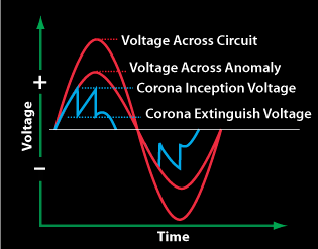
\includegraphics[width=\textwidth]{PartialDischarge}
    \caption{Partial Discharge}
    \label{fig:PartialDischarge}
\end{figure}

Partial discharge is a type of discharge in particular area occur because of transient in gas in oil insulation. Discharge occurs when current stress exceeds the defined critical value. The partial discharge level has a pronounced effect on the life of the current transformer\setlength{\parskip}{1em}.

As the current stress is increased, in the insulation system will result in Partial Discharge. As the current stress is reduced, Partial Discharge extinction will occur.
(MODIFIED)

The Partial Discharge cycle repeats rapidly during the peak values of a sine wave in current transformers. The excess energy dissipated during these repeating cycles causes deterioration of the insulation system resulting in premature failure of the Current Transformer.

Partial Discharge requires specialized equipment and cannot be characterized with standard dielectric testers. Partial Discharge can be minimized through the elimination of nano voids and contaminants during the design and manufacturing process. Construction materials and manufacturing process controls are designed for maximum product performance.

A BIL (Basic Insulation Level) rating on a Current transformer is an assurance that it will be able to routinely withstand power surges up to the given rating emanating from any number of common sources such as lightning, heavy motor start-ups, industrial load switching, grid overloads, \textit{etc}.

Recently, power grids, especially in metropolitan areas are reaching a level of saturation that results in a greater susceptibility to load variances, including lightning strikes. Consequently, AC switches and high voltage industrial equipment are exposed to voltage surges normally absorbed by the grid. BIL rated components are now being routinely specified for a much broader range of power control devices to greatly reduce the possibility of catastrophic system damage.

\begin{description}[style=nextline ]
 \item[Applied Voltage or Dielectric Test] A high voltage AC or DC test voltage is applied to the windings, and from the windings to ground. The test is designed to verify the adequacy of the system regarding coupling capacitance (AC) or resistance (DC).
 
 \item[Induced Voltage Test] The Induced Voltage Test reveals defects that might eventually result in a shorted turn and excessive excitation current. This test is important when winding layers are not properly insulated.
 
 \item[Partial Discharge (Corona) Test] The partial discharge test is a nondestructive method of identifying the potential for premature insulation breakdown. The test is capable of detecting small defects and nano voids in the insulation system that could lead to catastrophic transformer failure.
 \end{description}
 
Most of the research for Partial Discharge is done on medium voltage Current Transformers particularly on Cast epoxy resign. Need for analysis of High Voltage Current Transformers required to study effects of Partial discharge on performance. The insulation of CTs can be interested in the presence of common defects such as air bubbles or resin detachments at the interface between different parts of the component. The presence of such defects can be spotted during partial discharges tests \cite{sokolov1999effective}\setlength{\parskip}{0em}.
 
\subsection{On-line measuring system}

\subsubsection{On-Line partial discharge testing system for electrical systems}

There is \textbf{zero down time} associated with On-Line PD testing because the test is performed at normal operating voltage. Testing involves no external voltage or current sources\setlength{\parskip}{1em}.

Test equipment measures PD produced at voltages of 2400 volts and greater. The system is independent of load current. It is non-invasive testing that does not inject current into the system, nor does it subject the system to excessive voltage levels. Method is 100\% non-destructive and 100\% non-invasive systems.

The Online partial discharge testing gives warning of insulation failure so that maintenance plan can be done to avoid failure of instruments. Online testing gives the accurate condition of high voltage equipment including the effect of load, temperature and humidity. The on line testing are on destructive causing no interruption of service and performed under normal operating voltage, load and environmental conditions. No additional stress on the equipment under test no extra higher voltages stresses. In on line testing, the accuracy of PD measurement is more and more economical. The occurrence of PD can be located and can be repaired instantly.

The partial discharge activity will always lead to the dielectric breakdown of insulation inside the current transformer, The on line inspection techniques to measure partial discharge is developed by KEMA. A broad band high-frequency antenna is inserted inside to measure PD measurements during service. This technique is used for measuring PD in all HV equipment. The ultra high-frequency techniques are also used in many countries for on line detection. 

The diagnostic characteristics of current transformers and faulty insulation can be defined regarding partial activities and changes in capacitance and dielectric loss of defective area.

Contamination of defective area by dust particles, air bubbles in oil, the occurrence of small PD, destructive PD, progressive PD, will lead to the formation of gaseous. The gases thus formed will change the dielectric characteristics of insulation. The PD parameters can be concluded on Apparent charge magnitude, pulse repetition rate, discharge power, change in capacitance progressive PD.
 
The three methods for sensing PD used for on line measurements are acoustic, electromagnetic or frequency. In some cases, the combinations of these methods are 
also used as the diagnostic tool. The rough surface can be detected by using electromagnetic sensors, and the insulation strength can be detected by electric sensors and location of PD source by an acoustic sensor. The acoustic detection of partial discharge is an effective tool for the gaseous formed due to strong arcing in oil. The electric method can detect PD below 1000 pC, and acoustic method can detect above 10000 pC\setlength{\parskip}{0em}.

\subsubsection{Ultrasonic PD testing}
\setlength{\parskip}{0em}
Can pinpoint a suspected problem if the cable or accessory is not directly buried or is at least physically accessible.

The high-frequency ultrasonic components of PD are extremely short wave in nature, fairly directional and easy to isolate from background noise

The problem must be accessible.

\paragraph{Type of sensors advantages disadvantages\\}\setlength{\parskip}{1em}Electric direct connection to the test tap, or through high-frequency CT on the grounded wire, (\textquotedblleft Rogowski coils\textquotedblright) Additional sensors in bus duct, electrostatic shields, neural, \textit{etc}. High sensitivity Can be calibrated regarding apparent charge Approximate location of PD source All capabilities to trend data Use of PD pattern Recognition technology Sensors configuration can match for better noise rejection De-energizing for sensors installation.

Electromagnetic antenna easy to use possible assessing external PD problems including PD in the bushings Serving as noise (corona) channel High disturbances Only discharges of extremely high level can be detected Difficult to distinguish an equipment having problems from surrounding equipment.

Acoustic Piezo-accelerometer placed on transformer tank Easy to install Capability detecting acoustic emission magnitude and trend, Pulse repetition rate and trend Localizing a source of PD using signal time of arrival to different locations Low sensitivity Minimal detecting apparent charge \textgreater 10,000 pC Responded to rain, sleet, electrical disturbances in the station The level of signal depends on coupling between the sensor and surface Effect of design (variables inside the tank) on the propagation of sound wave.

The portable universal PD analyzer is used for different applications to detect PD in high voltage instruments transformers. The PD analyzer monitors waveforms for different power frequency simultaneously using many sensors and identifies PD pulses. The radio frequency pulses will identify the capacitance difference. The frequency band, 1 MHz to 20 MHz, can be selected by the sensors to detect PD in instruments. Electronic processing of signals, phase and frequency selection, time delay and signal comparison are done with the sensors simultaneously.

The modern techniques of on line measurement of PD gives a high sensitivity of PD measurement as comp aired to testing in the laboratory. The on line testing used as a diagnostic instrument. The on line testing can distinguish between small discharge and destructive discharge which affect electrical equipment to the critical status\setlength{\parskip}{0em}.

\subsection{Off line measuring system}

\subsubsection{Off-line testing techniques}
\begin{itemize}
\item Power Factor/Dissipation Factor Testing
\item Very Low-Frequency Testing (VLF)
\end{itemize}

\subsubsection{In-service testing techniques}
\begin{description}[style=nextline]
\item[Power Factor/Dissipation Factor Testing] This measurement is effective in identifying weak insulation and knowing reasons of potential hazards before the occurrence of a failure. Test process has no overstressed effect on insulation and gives the information of insulation strength of instrument.

\item[Very Low Frequency (VLF) Testing] This measurement process damages the insulation during the test. The supply with low frequency is applied to insulation. This process has the capability of locating potential failure at sites. VLF has the advantage of portability with low energy requirements, which results in much smaller test sets. Voltage is raised to above the Partial Discharge inception voltage which helps in creating partial discharge to occur.
\end{description}

\section[Effect of Partial Discharge on Electrical Equipments]{Effect of Partial Discharge on\\Electrical Equipments}
\subsubsection{Effect of partial discharge}
\begin{enumerate}
\item Partial discharge in Current transformers reduces dielectric strength of solid insulating resulting in the early break down of the instrument.

\item The partial discharge process can cause contamination of oil resulting in a change of insulating properties which will result in the early breakdown of the system.

\item Partial discharge measurement provides information on the aging effect on insulation which can help in deciding the life of the instrument.

\item Partial ~discharge ~identification ~indicates ~type ~of ~fault. The ~digital measurement system gives the inside information about discharge, the effect of environmental interference and strong information about maintenance required and quality of insulation. 
\end{enumerate}


\section{Predictions from Partial  discharge }
The partial discharge characteristics are different for different void conditions. The electrical trees formed depend on charge value and dimensions of voids. The amplitude of pulse, shape of the pulse width, rise and fall time depends upon the applied voltage and insulation strength. Discharge occurs in every half cycle due to the disturbances of voids\setlength{\parskip}{1em}.


Predictions of failure can be done from Electrical trees formed due to discharge in insulation. The penetration of tree in insulation, its branches, size, the formation of a void, dimensions of voids will help in assessing breakdown and collapse of an electrical instrument. 

Manufacturing process or insulation deterioration due to normal service operating conditions.

Partial discharge testing is a preventive detection tool which can alarm the potential failures due to insulation level of electrical equipment.

The Partial Discharge helps to identify discharge in insulation of cables, splices, transformers. The partial discharge testing is nondestructive testing\setlength{\parskip}{0em}.

\section{Study of Various Instruments Which Detects Partial Discharge in  High Voltage Instrument}

\subsection{Expert partial discharge analyzer with reflectometer - R2100}
R2100 shown as a complete kit with a variety of Partial Discharge Sensors
\begin{itemize}
\item Most Advanced PD Analyzer in the World
\item 12 PD Channels 
\item Noise Cancellation 
\begin{itemize}
\item Pulse Shape 
\item Pulse Polarity 
\item Pulse Comparison 
\item Time of Arrival 
\item Specialized software filters
\end{itemize}
\item TDR capability to assist in determining location of defect 
\end{itemize}

\begin{figure}[h!]
    \centering
    \begin{subfigure}[b]{0.32\textwidth}
        \centering
        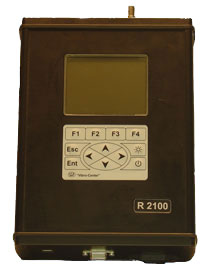
\includegraphics{251}
    \end{subfigure}
    \\
    \begin{subfigure}[b]{0.32\textwidth}
        \centering
        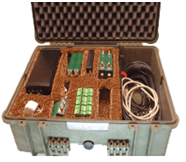
\includegraphics{252}
    \end{subfigure}
    \hspace{1cm}
    \begin{subfigure}[b]{0.32\textwidth}
        \centering
        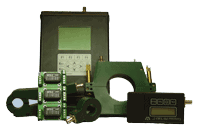
\includegraphics[height=4cm]{253}
    \end{subfigure}
    
    \caption{Expert Partial Discharge Analyzer with Reflectometer }
    \label{fig:Expert Partial Discharge Analyzer with Reflectometer }
\end{figure}

The instrument can measure external temperature, humidity. It has total 12 channels with the help of sensors. All PD channels have identical isolated input circuitry with protection and high pass filters. The frequency band is 0.5 to 10 MHz. This instrument eliminates the noise generated due to high voltage instrument in the substation. The instruments are fitted with noise filters. Almost all technologies that may found combined in different instruments on the market. PD channels may be flexibly configured to use one or another noise filtering technology or a combination of technologies \setlength{\parskip}{1em} \cite{gurin1975measurements}.

This instrument is an analyzer with the principle of the reflectometer. Reflectometer will help in identifying the defective location. This helps in identifying faults in long distance cables. The instrument is capable of recording up to three-time domain reflectograms per channel with different trigger levels. The trigger level may be automatically adjusted to signal level or pre-determined by the operator.

Partial data can be stored in this instrument. The instrument has 48 phase windows and 32 magnitude windows with a single dynamic range of 70 dB without gain adjustment. A full suite of software included that allows the user to download all data to a PC, perform analysis and present the data\setlength{\parskip}{0em}.

\subsection{Partial discharge analysis system}
 This instrument is an advanced system for analysis of partial discharge.
 
\begin{figure}[h!]
    \centering
    \begin{subfigure}[b]{0.30\textwidth}
        \centering
        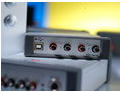
\includegraphics[height=3.5cm]{254}
    \end{subfigure}
    \begin{subfigure}[b]{0.60\textwidth}
        \centering
        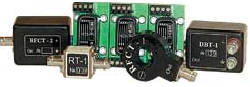
\includegraphics[height=3cm]{255}
    \end{subfigure}
    
    \caption{Partial Discharge Analysis System}
    \label{fig:Partial Discharge Analysis System}
\end{figure}

This instrument measures in high precision for high voltage equipment for insulation strength.Using galvanic isolation, it can minimize noise and most safe for measuring cable insulation for the distance of 2 kM. The instrument is light in weight and easy for portability\setlength{\parskip}{1em}. 

 
These are Vibro center equipment with Partial discharge sensors fitted inside. 

Sensors measure and diagnose partial discharge pulse. The sensors are perfect in the precision of measurement. Reliability of these instruments is very high. Sensors capture partial discharge pulses and give signal to the control unit. This instrument is designed for a load capacity of 50 $\Omega$ and can be attached directly to the measuring instruments\setlength{\parskip}{0em}.
 
\subsection{DB series sensors}
The DB series is used for high voltage equipment, bushings, current transformers. These sensors control dissipation factor and current and sense partial discharge phenomenon inside the current transformer and bushing. The insulation conditions inside the transformers are signaled with the sensors. The over voltage protection sensors are also fitted inside the instruments. These sensors are covered in the protective shield to avoid physical damage. The bushing of transformers is covered for protection as the high voltage equipment can undergo switching impulse and lightning threat. The switching impulse is not more than 1.3 kA for an instrument of 145 kV. The overvoltage protection is also sensed in the DB series. Various types of sensors depending on fitment requirement on instrument and bushing can be made suitable. These sensors are connected to PD measurement instrument.

The DB series sensors are designed based on the application are classified as:
\begin{itemize}
\item Operating voltage of bushing from 72 kV to 400 kV
\item As per the fitment on Equipment dimensions of sensors decided for ease fitment
\end{itemize}

\subsubsection{Sensor DB-1}
\begin{figure}[h!]
    \centering
    \begin{subfigure}[b]{0.49\textwidth}
        \centering
        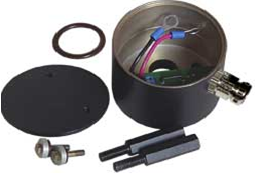
\includegraphics{256}
    \end{subfigure}
    \begin{subfigure}[b]{0.49\textwidth}
        \centering
        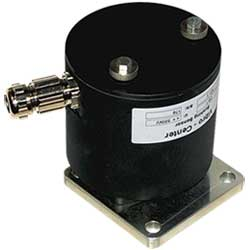
\includegraphics[height=4cm]{257}
    \end{subfigure}
    
    \vspace{3em}
    
    \begin{subfigure}[b]{0.49\textwidth}
        \centering
        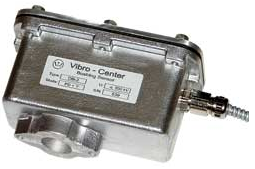
\includegraphics{258}
    \end{subfigure}
    \begin{subfigure}[b]{0.49\textwidth}
        \centering
        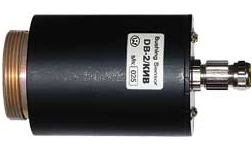
\includegraphics[height=4cm]{259}
    \end{subfigure}
    
    \caption{Sensor DB-1}
    \label{fig:Sensor DB-1}
\end{figure}

Sensor DB-1 are suitable for oil filled bushing transformers. These sensors are easy to mount on bushings of transformers for voltage above 132 kV. With mechanical fitting with the seal and study on bushings. The mechanical flange is provided for fitment on the bushing.

\subsubsection{DB-1 sensor structural variation}
These sensors are suitable for 110 kV operating voltage and easy for fitment on bushing fitted on transformer top cover.

These sensors are fitted in the metallic case and have protection for a high current pulse. The operating voltage above 66 kV \cite{gurin1993field}.

\subsubsection{Sensors for bushings of transformers}
The transformer bushing is filled with the oil and requires current monitoring sensors. These sensors have current measuring system and fitting arrangement on the body of transformers.

\begin{figure}[h!]
    \centering
    \begin{subfigure}[b]{0.49\textwidth}
        \centering
        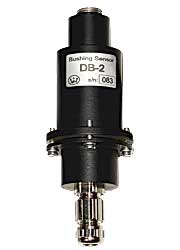
\includegraphics{2510}
    \end{subfigure}
    \begin{subfigure}[b]{0.49\textwidth}
        \centering
        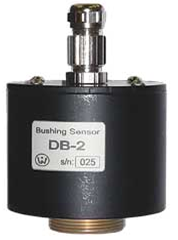
\includegraphics{2511}
    \end{subfigure}
    
    \caption{Sensors for bushings of transformers}
    \label{fig:Sensors for bushings of transformers}
\end{figure}

For the sensors which are produced by \textquotedblleft Trench,\textquotedblright \textquotedblleft GE\textquotedblright with the operating voltage of 300 kV and more it is these are possible to use the sensor that is shown in the picture. This sensor has a pilot thread of Ì 30 * 1,5 mm.

Three more sensor's varieties, which are produced by our firm, have a less spread, so they are not shown here. They have other types of mounting thread and the use of spring movable sensor contacts with the bushing test tap.

\subsubsection{Sensors DB-TT}
\begin{figure}[h!]
\centering
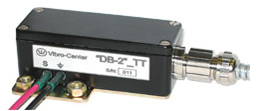
\includegraphics{2512}
\caption{Sensors DB-TT}
\label{fig:Sensors DB-TT}
\end{figure}

Sensors ~DB-2/TT ~these are ~used to ~know ~the insulation strength ~of ~current transformer. These sensors are fitted inside the terminal box.

\subsection{RFCT sensors}
These sensors are high-frequency transformers of current. Compared with usual transformer they separate in a current, which runs in the conductor, high-frequency impulses in the range from 0,5 MHz to 50 MHz from partial discharge. These sensors don’t record the current rippling of commercial frequency\setlength{\parskip}{1em}.

These are fitted on the grounding conductor, transformer neutral, and ground of the transformer tank, braiding ground of power cable, coupling capacitor ground and in the compensating circuit. 

The choice of the sensor mounting place depends on the controlled equipment type and task. For the task solution exact method of partial discharge recording is created. So the RFCT sensors embodiment is different, subject to the type of the seat for the sensor.

The special protective insulation, which is meant for protection of device measuring chain from external voltage, is not provided in the sensor’s construction. Therefore RFCT sensors could be mounted on the piece of equipment, which is the ground element or which is reliably attached to the ground only. In another case, it is necessary to envisage the use of additional insulation between the sensor case and the conductor line, in which the existence of partial discharge impulses is assumed\setlength{\parskip}{0em}. 

\begin{figure}[b!]
    \centering
    \begin{subfigure}[b]{0.49\textwidth}
        \centering
        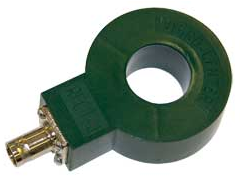
\includegraphics[width=\textwidth, height=6cm,keepaspectratio]{2513}
        \caption{RFCT-1 sensors }
    \end{subfigure}
    \begin{subfigure}[b]{0.49\textwidth}
        \centering
        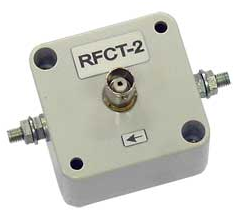
\includegraphics[width=\textwidth, height=6cm,keepaspectratio]{2514}
        \caption{RFCT-2 sensors }
    \end{subfigure}
    
    \begin{subfigure}[b]{0.49\textwidth}
        \centering
        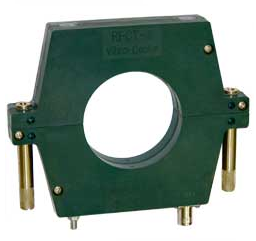
\includegraphics[width=\textwidth, height=6cm,keepaspectratio]{2515}
        \caption{RFCT-4 sensors }
    \end{subfigure}
    \begin{subfigure}[b]{0.49\textwidth}
        \centering
        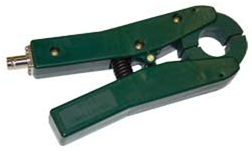
\includegraphics[width=\textwidth, height=6cm,keepaspectratio]{2516}
        \caption{RFCT-5 sensors }
    \end{subfigure}
    
    \begin{subfigure}[b]{0.49\textwidth}
        \centering
        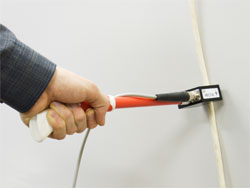
\includegraphics[width=\textwidth, height=6cm,keepaspectratio]{2517}
        \caption{RFCT-5 sensors }
    \end{subfigure}
    \begin{subfigure}[b]{0.49\textwidth}
        \centering
        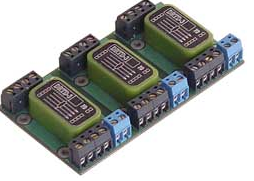
\includegraphics[width=\textwidth, height=6cm,keepaspectratio]{2518}
        \caption{RFCT-6 sensors }
    \end{subfigure}
    
    \caption{Types of RFCT Sensors to Detect Partial Discharge}
    \label{fig:Types of RFCT Sensors to Detect Partial Discharge}
\end{figure}

\subsubsection{RFCT-1 sensors}
The inside sensor core is implemented in the form of a hoop. The close gaps are necessary for sensitivity increasing of the measuring circuit. It can be explained by the range of the registered frequency. When mounting the sensor, it is necessary to break the metering circuit and to let the conductor through the sensor. The RFCT-1 sensor is connected with the device due to standard coaxial cable and BNC socket. Inside diameter of the sensor is 22 mm. 

\subsubsection{RFCT-2 sensors}
Constructively the sensor has a series of blocking capacitor of 6800 pF and pulse transformer inside. So RFCT-2 sensors are aimed at impulses registration of partial discharges in the high-voltage circuit breaker, the cell of the switchgear and control gear and in the cable lines, which are connected with it. Also, these sensors are used for impulses registration of partial discharges in other high-voltage equipment, where other RFCT sensors constructively cannot be used.

Electrically, the sensor does not let through power current through. It lets through partial discharge impulse only.

\subsubsection{RFCT-4 sensors}
The RFCT-4 sensor has the biggest inside diameter. These sensors are aimed at the installation on the transformer neutral and equipment ground bus. The sensor has a split case. It consists of 2 parts for the ease of installation on the bus, which has a rigid attachment. The sensor’s inside diameter is 68 mm.

Inside the sensor, there is a protective screen that may be connected to the ground through the ground bolt. This enables to improve the safety of measuring implementation.

\subsubsection{RFCT-5 sensors}
Constructively it is produced in the form of the current clamp and is aimed at the on-line control of the equipment insulation condition.

Sensors of this type are available with the device R-400. Originally this sensor is developed for the partial discharges measuring. However it can be used as the usual RFCT type sensor. 
 
The sensor is inside diameter, by which wire passes, is 24 mm.

\subsubsection{RFCT-6 sensors}
RFCT-6 sensors are aimed at online monitoring of electrical equipment (cable, cable box, \textit{etc}.) to identify partial discharges presence in equipment.

The RFCT-6 sensor is a partial discharges indicator only. Its data cannot be used for the appraisal of defect degree.

The sensor is connected to the device. The sensor is brought reasonably close to the conductor, in which the partial discharge detection is planned. The current direction in the wire must coincide with sensor pointer or be opposite. If turn the sensor at an angle of 90 degrees, then you cannot register the partial discharge.
 
The closer the sensor approach to conductor is the more amplitude on its output.

\subsection{DRTD-3 sensor}
A DRTD-3 sensor is aimed at the partial discharge recording in the stator winding of electric machine. As an antenna thermostats, which are put into electrical machine winding on the producer factory, are used. The sensor is included in the temperature measurement circuit break. The high-frequency component is single out from the complete signal from thermostats due to the sensor. High-frequency component carries the information about partial discharge in the winding. Sensor’s construction was designed in a way, that its involvement in the measurement circuit will not lead to significant accuracy in the process of the temperature measurement.

\subsection{KS-60 sensors}
\begin{figure}[h!]
\centering
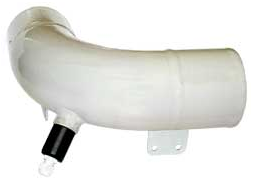
\includegraphics{2519}
\caption{KS-60 sensors}
\label{fig:KS-60 sensors}
\end{figure}

KS-60 ~sensor is created ~especially for the ~practical ~realization of the ~partial discharges method of recording in Transformers, or rather for the corona impulse tune-out. These impulses are a undesired signal. They are like a partial discharge impulse. Usually, it has a high amplitude and leads to the authenticity of monitoring system work of partial discharges in Transformers, and repeatable measurements by portable devices are inadmissibly low. So, despite these sensors, bulkiness, and difficulties with installation, the partial discharge monitoring system operation without using of KS-60 corona sensors (or such-like ) is impossible in the transformer.\\
 
As for physical aspect, the sensor of corona discharge impulses is aimed at the recording of the magnetic field tangential component, which appears the the transformer ~bushing ~bar ~while the high-frequency impulse ~flows ~through ~it. Depending on the direction of one impulse flow, inside or outside of transformer, signal polarity is changed on the sensor output.

\subsection{AR-1 sensor}
\begin{figure}[h!]
\centering
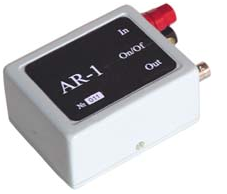
\includegraphics{2520}
\caption{AR-1 sensor}
\label{fig:AR-1 sensor}
\end{figure}

This sensor is aimed at the reference forming, which is necessary to partial discharge binding. The AR-1 sensors input signals could have different amplitude range, all the way from tens millivolts to supply voltage of 220 V. Rectangular impulse is formed in the sensor output. It has an even period as a input single. Input circuit and output circuit has a galvanic isolation for the voltage to 1500 V. Galvanic isolation allows excluding circuit interference between themselves and between the controlled object and measuring device. It is very important when the reference voltage for the phase binding is taken from another object made under high-voltage substation. Too small sensor input current, which numerically is equal to parts of microampere, extends the range of the sensor use. For example, when measuring on the transformer bushings, the sensor could be connected parallel to DBT-1 sensor, without error injection in the partial discharge measurements. The sensor could be used as an external synchronization of R400 device. The sensor has an inside power supply from two AA batteries. One complete set of batteries works for about 10 hours. The sensor is turned on and turned off by the power switch.

\subsection{RT-1 isolating transformer}
\begin{figure}[h!]
\centering
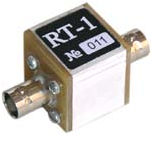
\includegraphics[scale=1.5]{2521}
\caption{RT-1 isolating transformer}
\label{fig:RT-1 isolating transformerr}
\end{figure}

This sensor is a high-frequency isolating transformer. The sensor is used in the partial discharge measuring circuit, where it may be circulating currents flow in the measuring and grounded circuits or between the measuring line. RT-1 sensor separates the high-frequency signal component of partial discharge from the signals of commercial frequency. The epoxy-filled isolating transformer is in the isolated case. It has a high-frequency transformation coefficient, which is equal to one.

\subsection{GKI-2 calibration oscillator}
\begin{figure}[h!]
\centering
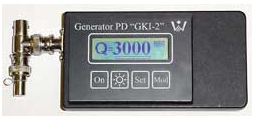
\includegraphics[scale=1.5]{2522}
\caption{GKI-2 calibration oscillator}
\label{fig:GKI-2 calibration oscillator}
\end{figure}

Small ~calibration ~oscillator ~GKI-2 ~is used for ~calibration of ~partial ~discharge registration circuit. Device injects electric charge into the controlled object and metering circuits. This makes it possible to calibrate a metering circuits given attenuation in the device before measuring. The injected charge circuit is connected through BNC connector on the left part of the device case.\\

The device injects a charge of 3nC into controlled object and metering circuit. The repetition frequency is 25 kHz. The leading edge of a pulse is about 5 ns. Calibration is in the sensitivity test of the measuring system. Sensitivity is set in nC/V. For example, the device registered the charge for 3nC, which is injected by the generator with an amplitude of 500 mV. Consequently the sensor's sensitivity is 3nC / 0.5V = 6nC/V.

\subsection{Ultrasonic and acoustic emission}
All operating equipment produces a broad range of sound. The high-frequency ultrasonic components of these sounds are an extremely short wave in nature, and a short wave signal tends to be fairly directional. It is therefore relatively straightforward to isolate these signals from background noises and detect their exact location. Also, as subtle changes begin to occur in electrical and mechanical equipment, the nature of ultrasound allows these potential warning signals to be detected early, before actual failure\setlength{\parskip}{1em}.

Airborne ~~ultrasound ~instruments, ~~often ~referred ~to ~as ~\textquotedblleft ~ultrasonic ~translators,\textquotedblright\\provide information two ways: qualitatively, due to the ability to \textquotedblleft hear' ultrasounds through a noise isolating headphone, and quantitatively, via incremental readings on a meter. This is accomplished in most ultrasonic translators by \textcopyright~2004 SKF Reliability Systems All Rights Reserved 2 MB04025 - Partial Discharge Analysis High voltage applications include insulators, cable, switchgear, buss bars, relays, contactors, and junction boxes. In substations, components such as insulators, transformers and bushings may be tested.

The method for detecting electric arc and corona leakage is similar to the procedure used to detect acoustic emissions from mechanical sources. Instead of listening for a rushing or rubbing sound, a user listens for a crackling or buzzing sound. In some instances, as in trying to locate the source of radio/TV interference or in substations, the general area of disturbance may be located with a gross detector such as a transistor radio or a wide-band interference locator. Once the general area has been located, the scanning module is utilized with a general scan of the area. The sensitivity is reduced if the signal is a too strong .electronic process called \textquotedblleft heterodyning,\textquotedblright which accurately converts the ultrasounds sensed by the instrument into the audible range where users can hear and recognize them through headphones \cite{sokolov1995experience}.

Although the ability to gauge intensity and view sonic patterns is important, it is equally important to be able to \textquotedblleft hear\textquotedblright the ultrasounds produced by the various equipment. That is precisely what makes these instruments so useful; they allow analysts to confirm a diagnosis on the spot by being able to discriminate among various equipment sounds.

The reason users can accurately pinpoint the location of a particular ultrasonic signal in a machine is due to its high frequency / short wavelength. Most of the sounds sensed by humans range between 20 Hz and 20 kHz (20 cycles per second to 20,000 cycles per second). They tend to be relatively gross when compared with the sound waves sensed by ultrasonic translators. Low-frequency sounds in the audible range are approximately 1.9 cm. to 17 meters in length, whereas ultrasounds sensed by ultrasonic translators are only 0.3 - 1.6 cm long. Since ultrasound wavelengths are magnitudes smaller, the ultrasonic environment is much more conducive to locating and isolating the source of problems in loud plant environments\setlength{\parskip}{0em}.

\subsubsection{Using ultrasonic and acoustic emission for partial discharge}
Ultrasonic testing is often used for evaluation at voltages exceeding 1,000 volts, especially in enclosed switchgear. This is especially useful in identifying tracking problems. In enclosed switchgear, the frequency of tracking greatly exceeds the frequency of serious faults, which can be identified using techniques such as infrared thermography\setlength{\parskip}{1em}.

When electricity escapes in high voltage lines or when it jumps across a gap in an electrical connection, it disturbs the air molecules around it and generates ultrasound. Often this sound will be perceived as a crackling or frying sound; in other situations, it will be heard as a buzzing sound.

There are three basic electrical problems that can be detected using ultrasound\setlength{\parskip}{0em}: 
\begin{description}
\item[Corona:] When the voltage on an electrical conductor, such as an antenna or high voltage transmission line exceeds the threshold value, the air around it begins to ionize to form a blue or purple glow.

\item[Tracking:] Often referred to as \textquotedblleft baby arcing,\textquotedblright follows the path of damaged insulation.

\item[Arcing:] An arc occurs when electricity flows through space. Lightning is a good example. 
\end{description}

The process can be used to detect both end winding (Phase to Phase) and slot section (Phase to Earth) discharge.

\subsubsection{Partial discharge pattern recognition of current transformers using an ENN  extension neutral network}
Extension-neural-network (ENN)-based recognition method to identify the partial-discharge (PD) patterns of high-voltage current transformers (HVCTs). First, a commercial PD detector is used to measure the three-dimensional (3D) PD patterns of HVCTs, then three data preprocessing schemes that extract relevant features from the raw 3-D PD patterns are presented for the proposed ENN-based classifier. Than traditional neural networks. The ENN has the advantages of high accuracy and noise tolerance, which are useful in recognizing the PD patterns of electrical apparatus. 

\subsubsection{Partial discharge sensors and bushing conduction current sensors, that are being produced by Vibro-Center}
Primary sensors are the base of all measuring diagnostic system. Functionality and operating efficiency of all measuring systems depend on sensors precision and reliability.

Vibro-Center produces a wide variety of sensors for the control operation of the equipment, which registers partial discharges. All these sensors are meant for registration of \textquotedblleft electric\textquotedblright partial discharges in high-voltage power equipment. All these sensors are aimed at working with a standard load of 50 $\Omega$, so they can be used for working with measuring devices that are produced by other companies. A current transformer is very important apparatus in electrical power system the measurement and protection. Partial discharges in a current transformer are often a predecessor of a serious fault. For this reason, partial discharge measurements are nondestructive diagnostic tool to monitor the insulation condition of a current transformer. The simple Partial Discharges (PD) detection is not enough to decide against intervening, so the localization is necessary to assess the risk and to plan corrective actions.

\pagebreak 
\section{Research Gap}
Various literature is available on partial discharge phenomenon, causes, measurement, and testing of electrical equipment. But very few data available on high voltage oil filled current transformers 145 kV, where the primary current is very high from 100 Amp to 3000 Amp\setlength{\parskip}{1em}.
 
The effect on Insulation medium used has high electrical stress due to high current capacity. The failure of current transformers in the system will lead to the breakdown of the complete system. Hence need for analysis is required to study the effect of Partial Discharge on High Voltage Current Transformers 145 kV up to 3000 Amp.

There is need to develop and study some models in Simulink to verify and analysis Partial discharge pulses. As Partial Discharge phenomenon starts because of contamination in insulating material or presence of a void in insulating material, due to both insulation strength gets weakens and discharge of charge starts at weak points. Hence it is necessary to study the effect various voids on the performance of current transformers during steady state conditions and short circuit and transient conditions. The presence of voids in the insulating material represents capacitance which causes discharge phenomenon in the insulating material. The study is required for different waveforms for different void conditions, nature of pulses, amplitude, wavelength from the Simulink model during steady state and short circuit and transient conditions. Need to study the difference in ratio error, phase error for accuracy test during steady state and transient conditions.

Thus need for study effect of voids on partial discharges, the study of mathematical model and effect of steady state conditions and short circuit and transients conditions and analysis of waveforms to make improvements in servicing, manufacturing and designing of high voltage oil filled current transformers for un-interruption in power supply.
\setlength{\parskip}{0em}

\chapter{SYSTEM DEVELOPMENT}
%system developement

To study the partial discharge analysis in oil filled current transformers, the following system was studied

\begin{enumerate}
\item Mathematical Model for oil filled current transformers
\item Mathematical Model for void in oil insulation
\item Simulation Model in Steady State 
\item Simulation Model in Short Circuit and Transients 
\end{enumerate}

The system was developed to make the mathematical model of oil filled current transformers represent primary and secondary resistance and inductance. This will help in the representation of any current transformer with respective values. This will help in calculating apparent charges and discharge for particular dimensions of voids\setlength{\parskip}{1em}.

The ~void ~is ~considered ~in ~oil ~and ~paper insulation which will give values of capacitance for different sizes of voids. The capacitance values will help in Simulink model for the study of partial discharge during steady state and transient conditions.

A simulation model was considered to co relate relation of void dimensions and the condition of working instrument during normal steady state and due to transient conditions. Two different models in MATLAB/Simulink were considered for steady state condition and short circuit or during transients. A void of various size and shape were considered to study the effect of partial discharge pulse\setlength{\parskip}{0em}.

\section{Computational Models}
\subsection{Simulation model for oil filled high voltage current transformers in steady state condition}

\begin{figure}[h!]
\centering
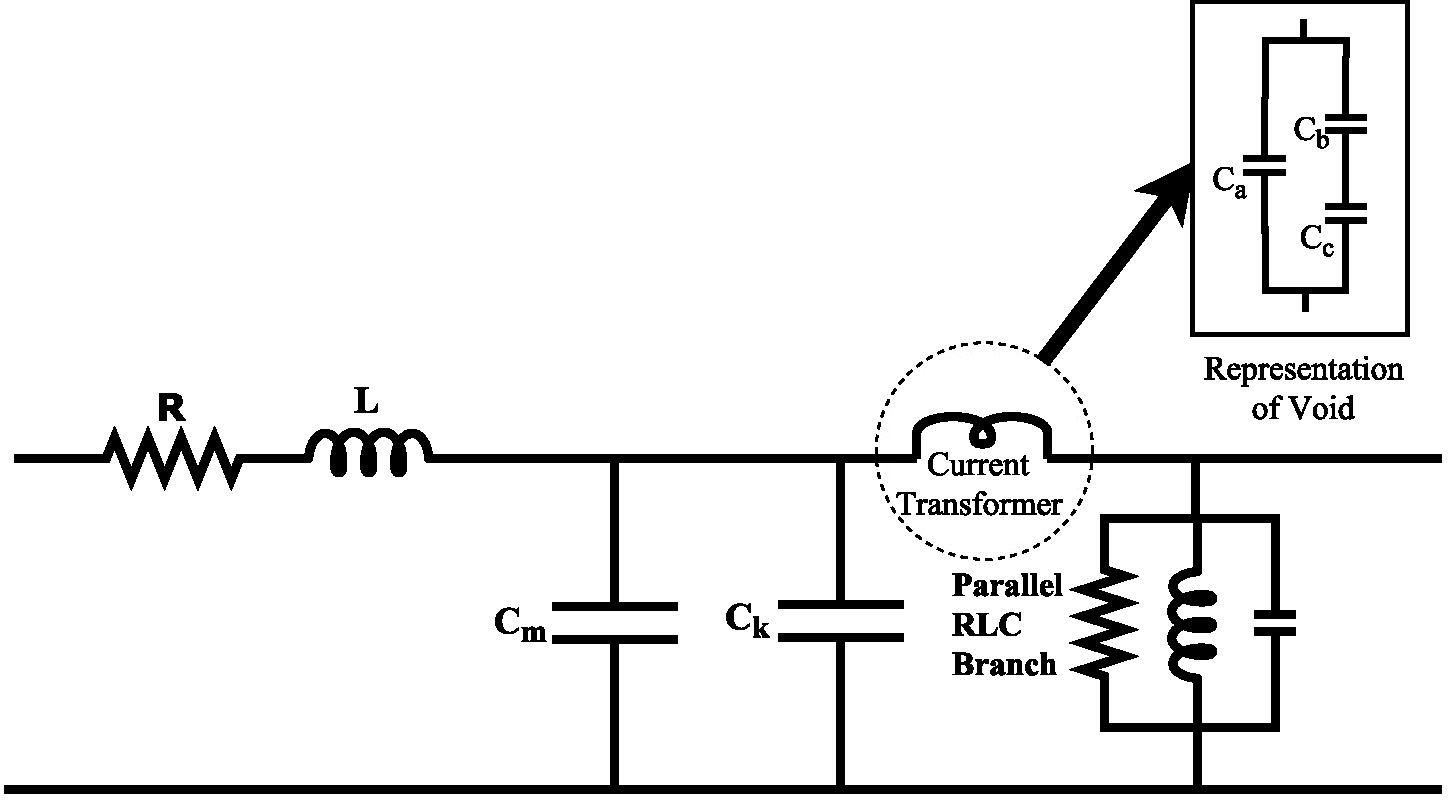
\includegraphics[width=\textwidth]{SimulationModelforHighVoltageCurrentTransformers}
\caption{Simulation Model for High Voltage Current Transformers in Steady State Condition}
\label{fig:Simulation Model for High Voltage Current Transformers in Steady State Condition}
\end{figure}

To study partial discharge pulses due to various sizes of voids capacitor circuit is considered with capacitance $C_b$ and $C_c$ in series and $C_a$ in parallel\setlength{\parskip}{1em}.

The void will represent various capacitance which is named as $C_a$, $C_b$, $C_c$. $C_a$ is the capacitance of discharge free oil insulation of the current transformer. $C_b$ is capacitance in series of void C under consideration. $C_c$ is the capacitance of void.
 
The values of capacitance are $C_a > C_b > C_c$

For the Simulink model to run during steady state conditions, various sizes of voids are considered. The capacitance $C_a$, $C_b$, $C_c$ are calculated for each size of voids. The sample size for the cube for calculation purpose considered as 20x20x6 mm. The detail values of capacitance are shown in the table \ref{table:Values of Capacitance for Different Void Sizes}.

Simulation Model for High Voltage Current Transformers in Steady State Condition derived and concluded, The values of partial discharge depends upon the size of the void, applied voltage and dielectric strength of insulating material From the waveforms generated for the various magnitude of the void, magnitude, number of PDs, Distribution of discharge were studied\setlength{\parskip}{0em}.

\subsection[Simulation model for high voltage current transformers in short circuit and transient condition]{Simulation model for high voltage current\\transformers in short circuit and\\transient condition}

\begin{figure}[h!]
\centering
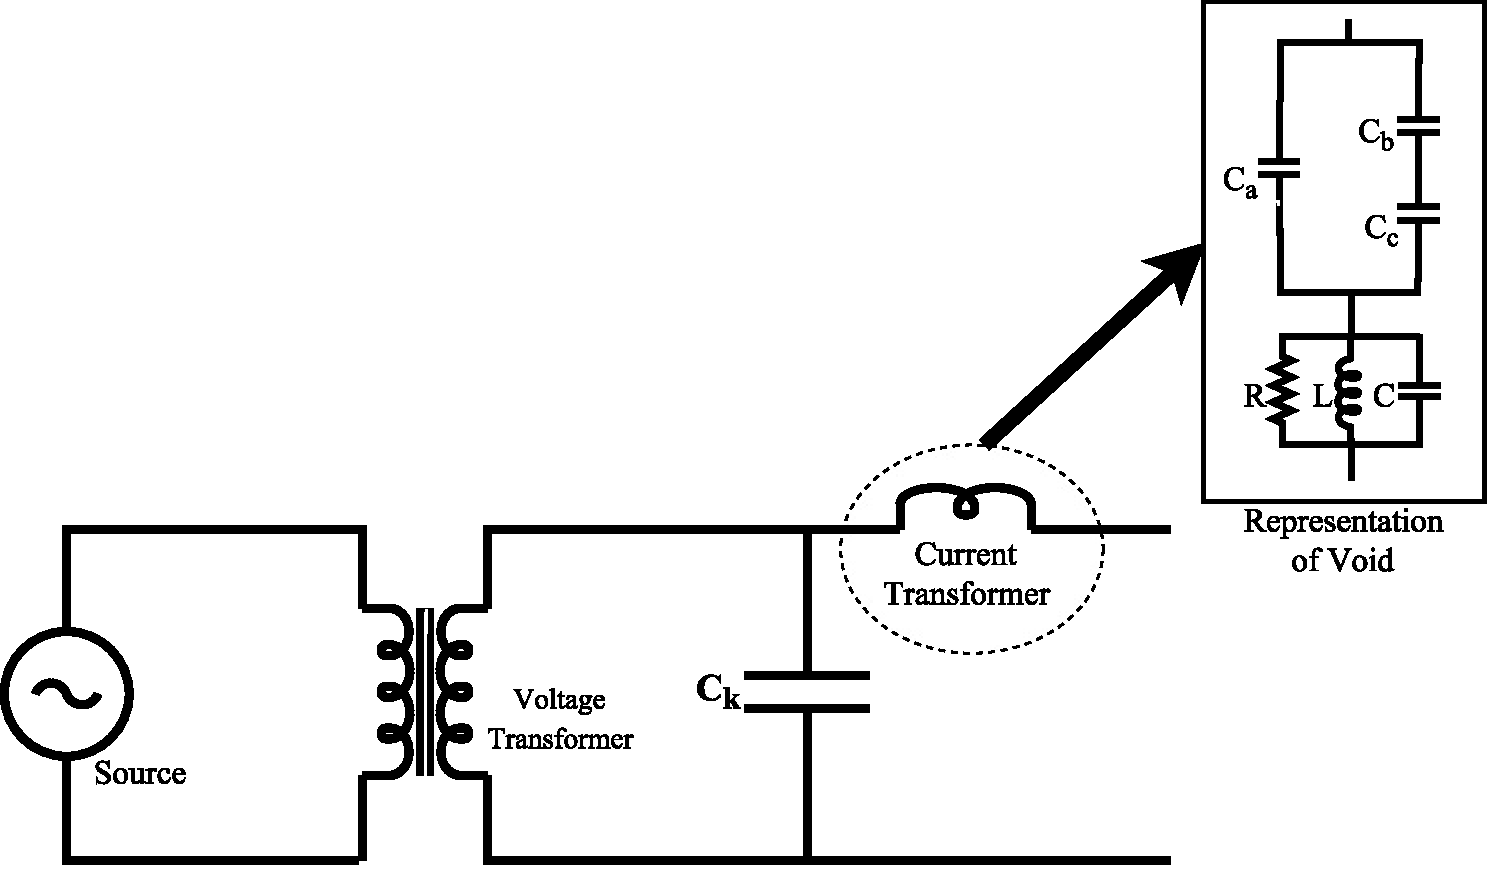
\includegraphics[width=\textwidth]{SimulationModelofPDMeasurementinTransientCondition}
\caption{Simulation Model of PD Measurement in Transient Condition}
\label{fig:Simulation Model of PD Measurement in Transient Condition}
\end{figure}

To Partial discharge process has been initiated for voltage 145 kV and various sizes of voids. Simulink model was run for various void dimensions. Calculated Capacitance values for $C_a$, $C_b$, $C_c$ were given to the circuit. Partial discharge pulses were recorded and studied. With the short circuit and transients, the partial discharge density and magnitudes are very high and thick. The waveforms will show this phenomenon on partial discharge waveforms.

\pagebreak 
\section{Analytical Models}
\subsection[Mathematical model of high voltage current transformers]{Mathematical model of high voltage\\current transformers}
Models for oil filled current transformers with specifications mentioned above are considered for making an analytical model.

\begin{figure}[h!]
\centering
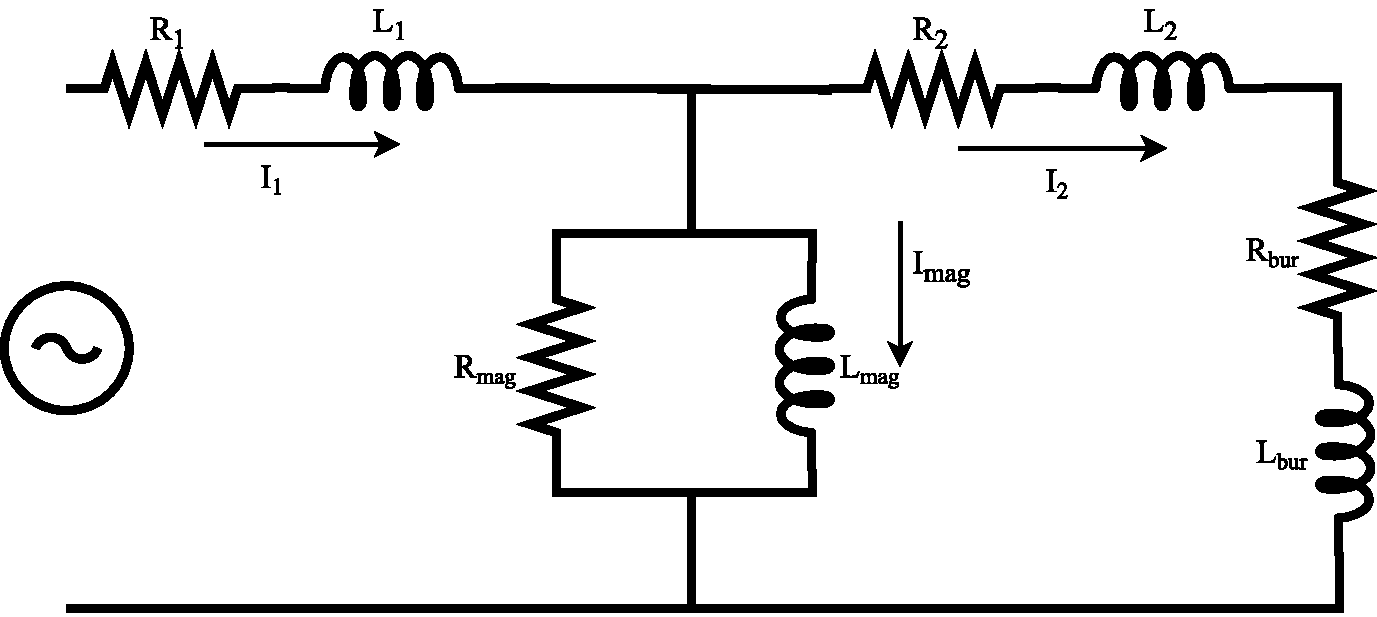
\includegraphics[width=\textwidth]{MathematicalModelofHighVoltageCurrentTransformer}
\caption{Mathematical Model of High Voltage Current Transformer}
\label{fig:Mathematical Model of High Voltage Current Transformer}
\end{figure}

\begin{tabbing}
paragraph \quad 	\= 	paragraph \kill
$R_1 L_1$			\> - Primary leakage impedance \\
$R_2 L_2$ 			\> - Secondary leakage impedance\\
$R_{bur} L_{bur}$	\> - Burden impedance\\
$i_{mag}$			\> - Current derived by the magnetizing branch\\
$i_{fe}$			\> - Current derived by the branch representing core losses.
\end{tabbing}

$i_p - i_{mag}+ i_{sec}$

The flux changes with magnetic current. Writing the equation for current flowing in the magnetizing path with initial data and \textit{w.r.t} time new. The flux will be variable\setlength{\parskip}{1em}.

The mathematical model represents electrical circuit of current transformers with primary and secondary impedances, current in various branches and core loss in the circuit.

$R_1 L_1$ is the resistance and inductance of primary winding, which is 145 kV line and carrying current from 100 A to 3000 A depending upon circuit and acts as the primary of current transformers.

$R_2 L_2$ is resistance and inductance of secondary winding which is carrying a current of 1 A or 5 An in the secondary of current transformers.
 
The magnetizing of cores are represented by a middle link with magnetizing current and electric burden on the system.

This mathematical circuit helps in evaluating the performance of the current transformer in normal working condition and during a short circuit and transient conditions \cite{harrold1985influence}.

With this mathematical representation, any current transformer can be represented in a mathematical model with the values of circuit impedance of the primary and secondary circuit. This will help mathematically to derive the effective performance in the long term\setlength{\parskip}{0em}.  

\subsection{Mathematical model of void in oil insulation}
\subsubsection{Partial discharge equivalent circuit model}
The phenomenon of partial discharge initiates in the voids present in insulating material oil or paper in 145 kV current transformers. The dielectric strength of the insulating material is very high which can sustain electrical stresses inside the instruments. With the presence of a void, the dielectric strength gets reduced, and electric discharge gets initiated. A common source of Partial discharge in solid dielectrics are voids present in the High Voltage Current Transformers. Since voids are the main source of partial discharges, it is necessary to study a mathematical model of partial discharge inside insulation oil or paper. With the period and continuous electrical stresses, insulation deterioration starts and breaks when electrical stress in the void is more than the dielectric strength of the complete insulating material. The size of void plays a major role in discharge phenomenon, and bigger size of voids can lead to complete breakdown of current transformers.\\

For the study purpose, we have considered void in the insulating material oil and paper with specific dimensions. In relation to void dimensions, the capacitance values are calculated. 

\begin{figure}[h!]
\centering
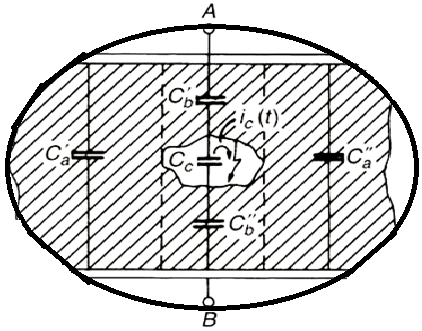
\includegraphics[width=\textwidth]{DielectricMaterialWithaCavity}
\caption{Dielectric Material With a Cavity}
\label{fig:Dielectric Material With a Cavity}
\end{figure}

Figure \ref{fig:Dielectric Material With a Cavity} represents a gas filled void in as capacitor. The partial discharge in void depends on the relative permittivity of the material used and depend on the electrical stress generated. The various capacitance is formed in the geometry sample under consideration.

$C_c$ is the void capacitance\\
$C_b$ is the series capacitance with void\\
$C_a$ is the capacitance of insulation \\
$C_b'$ is capacitance between void and electrode A\\
$C_b''$ is capacitance between void and electrode B\\
Two sides of healthy capacitance are represented by $C_a'$ and $C_a''$. \\
Total capacitance of healthy insulation is $C_a$= Capacitance of both sides of voids, addition of $C_a$ and $C_b$\\
And Similarly, the capacitance in series with void is calculated with capacitance in parallel $C_b = C_b' C_b''/ C_b'+C_b''$.\\
In general $C_a \gg C_b \gg C_c$

\begin{figure}[h!]
\centering
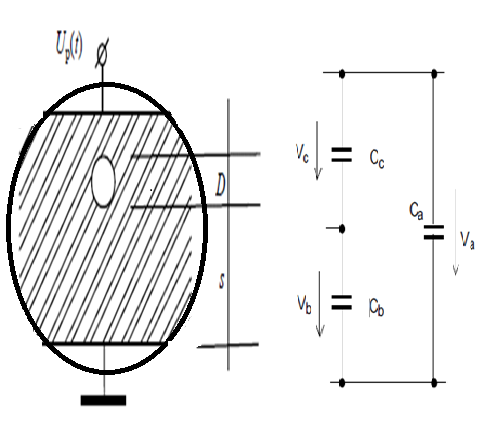
\includegraphics[width=\textwidth]{EquivalentCircuitofaCavityEnclosedinaSolidInsulatingMaterial}
\caption{Equivalent Circuit of a Cavity Enclosed in a Solid Insulating Material}
\label{fig:Equivalent Circuit of a Cavity Enclosed in a Solid Insulating Material}
\end{figure}

The classical model (or abc model or the Gemant- von Philippo model) is given schematically in Fig. 1. The void taken for calculating capacitance is represented as $C_a$ the capacitance of Insulation, $C_b$ as the capacitance of next to void and $C_c$ is the capacitance of void. The voltage across the cavity can be given by 

\begin{equation}
V_c = V_a \frac{C_b}{C_b + C_c}
\end{equation}

The important factor for partial discharge characteristics is void parameters. Partial discharge pulses vary according to the size of the void. Voids can be represented as cylindrical, cubical, rectangular or of irregular shape, \textit{etc}. The capacitance value will change based on the dimensions of voids hence partial discharge, and related parameters will change.

\begin{figure}[h!]
\centering
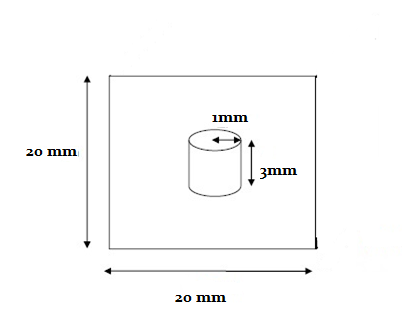
\includegraphics[width=\textwidth]{RepresentationofVoidinOilFilledCurrentTransformer}
\caption{Representation of Void in Oil Filled Current Transformer}
\label{fig:Representation of Void in Oil Filled Current Transformer}
\end{figure}

The object is made up of impregnated paper and represented as three capacitors. Voids are considered in this insulation as per above considerations three capacitance are calculated $C_a$, $C_b$ and $C_c$.

The relative permittivity of Dielectric material considered in this exercise are :

Impregnated Paper Relative permittivity $\varepsilon_r = 5$\\
Free Space Relative permittivity $ \varepsilon_0 = 8.852 \times 10^{-12} F/m$\\
Gap between electrodes $d = 0.005 m$

\subsubsection{Electrical circuit illustrating the partial discharge measurement}
Measurement of Partial Discharge is done to ascertain the healthy condition of current transformers. The test current transformers are connected to the measuring circuit and will measure PD in nano Coulomb. The normal, acceptable limit is up to 10 pC. The impedance of test measuring equipment also has the effect on calculating PD parameters. The circuit diagram shown in figure 4 represents Vs. voltage source, Z impudence of test circuit \cite{harrold1985influence}.

\begin{figure}[h!]
\centering
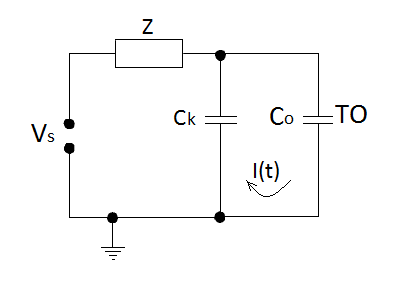
\includegraphics[width=\textwidth]{ElectricalCircuitforPrincipleofPDMeasurement}
\caption{Electrical Circuit for Principle of PD Measurement}
\label{fig:Electrical Circuit for Principle of PD Measurement}
\end{figure}

When the phenomenon of discharge occurs the voltage across test object reduces by $\Delta V$ Capacitance of test CT can be defined as 

\[
C_o \approx C_a + C_b~~~~~~\text{(assuming } C_c \text{ to be negligibly small).} 
\]

If $C_k \gg C_o$ the charge transfer is given by 

\begin{align}
q &= \int i(t) dt \approx (C_a + C_b)\Delta V \\
\text{Now~~} \Delta V &= \frac{C_b}{C_a + C_b} \Delta V_c \\
\Delta V &= \frac{q}{C_a + C_b}\\
i.e. &~~~~\frac{q}{C_a + C_b} = \frac{C_b}{C_a + C_b}  \Delta V_c \\
q &= C_b \Delta V_c
\end{align}

$q$ in above equation is defined as apparent charge and $\Delta V_c$ voltage drop across the cavity in the insulating material

\begin{figure}[h!]
\centering
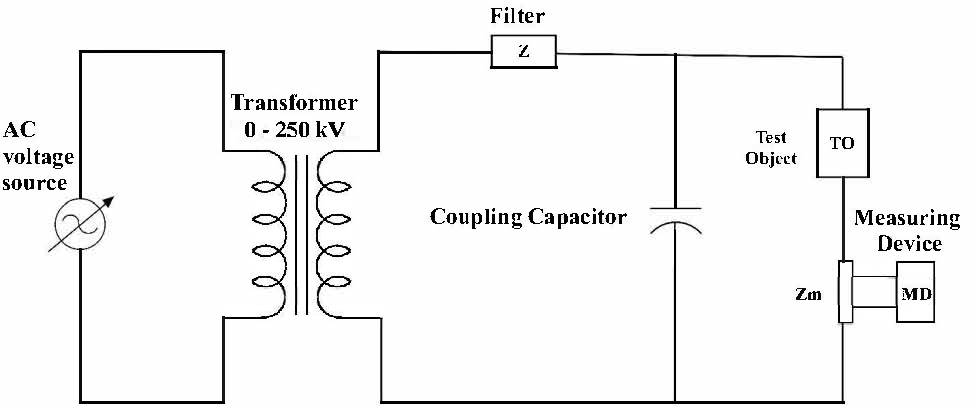
\includegraphics[width=\textwidth]{ConventionalPDmeasurement}
\caption{Conventional PD measurement}
\label{fig:Conventional PD measurement}
\end{figure}

The partial discharge phenomenon initiates the breakdown of dielectric and leads to the formation of the arc which is flow of electrons across the void. The electronics flow faster rate and can be represented in the form of pulses in the waveform. The flow of electronics which has –ve charge generate discharge $i = dq / dt$. During partial discharge phenomenon, also positive ion is created, and disturbances in voids are created. This process is detected by the coupling capacitor in the circuit\setlength{\parskip}{1em}.

Partial discharges in the current transformers depend upon capacitance values of voids and insulating material.
 
In this experiments, various sizes of voids are considered such as cylindrical, rectangular, square, ellipse with various dimensions. The cube sample considered is $20 \times 20 \times 6$

The capacitance $C_a$, $C_b$, $C_c$ are formed in sample size are considered, and values of capacitance are calculated with the formulas : 

\begin{align}
C_c &= \frac{\varepsilon_0 \times r^2 \times \pi}{h}\\
C_b &= \frac{\varepsilon_0 \times \varepsilon_r \times r^2 \times \pi}{d - h}\\
C_a &= \frac{\varepsilon_0 \times \varepsilon_r \times (A - r^2 \pi)}{d}
\end{align}

The voltage applied to current transformer test object 145 kV and 50 Hz frequency. To study capacitance values are calculated in the form of $C_a$, $C_b$, $C_c$. enclosed shows all calculated values. 

In the circuit used for calculating partial discharges, the Test instrument is considered, and components values are considered in simulation circuit.

\begin{tabular}{l  l}
1. High Voltage Transformer		&: Primary 230 V; Secondary 145 kV\\
2. Value of Measuring Capacitor	& : 400/1600 pF\\
3. Value of Coupling Capacitor	& : 1000 $\mu$F\\
\textbf{RLC values of Detector circuit} & {}\\
4. Resistance					& : 500 $\Omega$\\
5. Inductance	 				& : 0.065 mH\\
6. Capacitance 	 				& : 0.47 $\mu$F
\end{tabular}

Simulation has been done for high voltage current transformers to evaluate the performance during Steady State Condition and Short Circuit and Transient conditions. The performance has been evaluated by considering various voids and calculating the capacitance $C_a$, $C_b$, $C_c$. With this values put in Simulation model, the performance in the form of the waveform can be generated in Matlab\setlength{\parskip}{0em}.

\section[Manufacturing Processes and Actions to Avoid Partial Discharge]{Manufacturing Processes and Actions to\\Avoid Partial Discharge}
Partial Discharge measured in Current Transformer acceptable limit is between 5 pC to 10 pC Out of the results measured segregated CT where Partial Discharge is more than 10 pC After the Analysis, following reasons observed which lead to higher PD

\begin{enumerate}
\item High Vacuum Level
\item low Temperature
\item High Oil Flow Rate
\end{enumerate}

During manufacturing process the parameters specified are :

Vacuum Level $5 \times 10^{-4} = 0.5 mbar$\\
Temperature 138\textdegree C \\

Oil flow rate Initial for 6 hrs 0.5 lit/hr\\
Middle for 8 hrs 4 lit/hr\\
Final for 8 Hrs 14 lit/hr\\
Analysis of Partial Discharge in Current Transformers\\
a) Low vacuum level less then 0.5 mbar\\
Low vacuum extracts less moisture.\\
Retained moisture leads to Partial Discharge.\\
Evacuation system is designed for high vacuum and low temp.\\
If vacuum is high, then evaporation rate is less then100\textdegree C\\
Dielectric strength of impregnated insulation should be more, if not voids will be formed \\
b) Low temp of oil less then138\textdegree C\\
If the temperature of the oil is less then138\textdegree C, moisture contents in the insulation will not be removed and can form voids in the insulating material.

The insulation paper layers are around 22 nos, the temp must reach the inner most layer and remove the moisture contents.

The Nonremoval of moisture of insulating material will reduce the insulating strength and can discharge with high magnitude pulses.

c) Effect of High Oil flow rate
During the filling of transformer oil in current transformer care should be taken to control flow rate otherwise chances of forming bubbles in oil and air may trap inside. 

Hence oil flow should be slow to the extent paper absorbs oil. If it is more paper will not absorb oil completely and simultaneously air bubble formation in the oil tank.

The elasticity of paper that provides compression pressure on the inner layer will not allow the air to trap. The paper used in the sequence of Non stretched, Light Stretched and crepe paper.

The quality of insulation paper should match the absorption with the rate of oil filled in current transformers. If the absorption rates are not matched, there will be chances of forming voids and Voids are the potential for partial discharge.

\subsection{Service experience analysis}

\subsubsection{Case 1}
Current Transformer, 145 kV oil, filled after 15 years working in substation due to the explosion of the bushing. This failure has resulted in damage to secondary winding insulation, contamination of the toroidal cores and shell assembly, rupture of porcelain and contamination of the oil.
 
This case is the total breakdown of insulation dielectric strength and the result of persistent partial discharge at some area in oil, paper, copper, bushing, core or another part. 

\subsubsection{Case 2}
The on line current transformer after long service was taken for partial discharge measurement and taken for life assessment. 

The oil insulation must have undergone various transient conditions during long term operation. The deterioration of insulation strength can be evaluated from a breakdown voltage and measurement of Tan delta.

BDV of oil 90 kV\\
Tan delta 0.00019\\

The Service condition has shown good results of the insulation strength of oil.\\
The current transformer oil contains the following chemicals:\\

\begin{tabular}{| l l | l l | l l | l l | }
\hline
$H_2$ & :0.034 & $CH_4$ & :0.52 & $C_2H_2$ & :0.162 &  $C_2H_4$ & :0.21\\ \hline
$C_2H_6$ & :0.60 & $CO$ & :0.067 & $CO_2$& :0.12 & $N_2$ & :4.7 \\ \hline 
\end{tabular}

\subsection{Specifications of current transformers}
Current Transformer 1
\begin{table}[h!]
\caption{Specification of Current Transformer 1}
\label{table:Specification of Current Transformer 1}
\centering
\begin{tabular}{|l|c|}
\hline 
CT Ratio &  3000/1  \\ \hline 
Core Size & $225 \times 275 \times 50$ \\ \hline 
No. of turns on Secondary  & 3000 \\ \hline 
Burdon & 30 VA  \\ \hline 
KPV (V)  & 20 mA @vk/2 \\ \hline 
Resistance  & 12 $\Omega$\\ \hline 
Excitation current & 12 mA \\ \hline 
ISF  & 5 \\ \hline 
Accuracy Class  & 0.5 \\ \hline 
\end{tabular} 
\end{table}

\clearpage
Current Transformer 2
\begin{table}[h!]
\caption{Specification of Current Transformer 2}
\label{table:Specification of Current Transformer 2}
\centering
\begin{tabular}{|l|c|}
\hline 
CT Ratio &  2400/1  \\ \hline 
Core Size & $220 \times 400 \times 45$ \\ \hline 
No. of turns on Secondary  & 2400 \\ \hline 
Burdon & No burdon  \\ \hline 
I excitation   & 100 vk \\ \hline 
Resistance  & 18 $\Omega$ \\ \hline 
Excitation current & 28 mA \\ \hline 
ISF  & 5 \\ \hline 
Accuracy Class  & PS \\ \hline 
\end{tabular} 
\end{table}

Current Transformer 3
\begin{table}[h!]
\caption{Specification of Current Transformer 3}
\label{table:Specification of Current Transformer 3}
\centering
\begin{tabular}{|l|c|}
\hline 
CT Ratio &  200/1  \\ \hline 
Core Size & $220 \times 405 \times 40$ \\ \hline 
No. of turns on Secondary  & 200 \\ \hline 
Burdon & No burdon  \\ \hline 
KPV (V)   & 20 mA vk/2 \\ \hline 
Resistance  & 11 $\Omega$\\ \hline 
Excitation current & 12 mA \\ \hline 
ISF  & 5 \\ \hline 
Accuracy Class  & 0.2 S \\ \hline 
\end{tabular} 
\end{table}

\clearpage
Current Transformer 4
\begin{table}[th!]
\caption{Specification of Current Transformer 4}
\label{table:Specification of Current Transformer 4}
\centering
\begin{tabular}{|l|c|}
\hline 
CT Ratio &  600/1  \\ \hline 
Core Size & $215 \times 300 \times 25$ \\ \hline 
No. of turns on Secondary  & 150 \\ \hline 
Burdon & No burdon  \\ \hline 
I excitation   & 100 vk \\ \hline 
Resistance  & 0.2 $\Omega$ \\ \hline 
Excitation current & 340 mA \\ \hline 
ISF  & 5 \\ \hline 
Accuracy Class  & 5P \\ \hline 
\end{tabular} 
\end{table}

\newgeometry{left=1.5in,right=1in,top=0.8in,bottom=1in}
\begin{table}[h!]
\caption{Results of Accuracy testing of Current Transformers in Steady State and transients}
\label{table:Results of Accuracy testing of Current Transformers in Steady State and transients}
\renewcommand{\arraystretch}{1.3}
\centering
\begin{tabular}{|>{\centering\arraybackslash}m{0.6in}|>{\centering\arraybackslash}m{0.5in}|>{\centering\arraybackslash}m{0.6in}|>{\centering\arraybackslash}m{0.8in}|>{\centering\arraybackslash}m{0.7in}|>{\centering\arraybackslash}m{0.8in}|>{\centering\arraybackslash}m{0.7in}|}
\hline 
\multicolumn{3}{|c|}{} & \multicolumn{2}{c|}{Steady state} & \multicolumn{2}{c|}{Transients} \\ \hline 
Ratio & Burden  & Primary Current & Ratio Error  & Phase Error  & Ratio Error  & Phase Error  \\
(Amp/) & (VA) & (\%) & (\%) & minutes & (\%) & minutes \\ \hline \hline
\multirow{8}{*}{3000/1} & \multirow{4}{*}{30} & 120 & 0.342 & 0.56 & 2.345 & 3.423 \\ \cline{3-7}
 &  & 100	& 0.331 & 0.67 & 2.456 & 3.674\\ \cline{3-7}
 &  & 20  & 0.129 & 2.56 & 1.341 & 2.874 \\ \cline{3-7}
 &  & 5   & 0.012 & 3.98 & 1.456 & 2.712\\ \cline{2-7}
 & \multirow{4}{*}{7.5} & 120&0.256 & 0.35 & 2.023 & 4.512 \\ \cline{3-7}
 & & 100&0.237 & 0.45 & 2.402 & 4.521 \\ \cline{3-7}
 & & 20 & 0.148 & 0.56 & 1.890 & 2.98 \\ \cline{3-7}
 & & 5& 0.126 & 0.21 & 1.562 & 2.453 \\ \hline \hline
2400/1 & 0 & 100 & -0.034 & 0.96 & 5.670 & 15.59 \\ \hline \hline
600/5 & 10 & 100 & 0.007 & 0.29 & 3.15 & 9.23 \\ \hline \hline
\multirow{8}{*}{200/1} &\multirow{4}{*}{30} & 120 & 0.116 & 0.33 & 1.568 & 1.89 \\ \cline{3-7}
& & 100 & 0.112 & 0.34 & 1.558 & 1.87\\ \cline{3-7}
& & 20 & 0.076 & 1.78 & 2.321 & 4.56\\ \cline{3-7}
& & 5 & 0.053 & 3.47 & 2.291 & 9.37 \\ \cline{2-7}
& \multirow{4}{*}{7.5} & 120 & 0.158 & 0.18 & 1.628 & 1.75\\ \cline{3-7}
& & 100 & 0.157 & 0.21 & 1.601 & 1.71 \\ \cline{3-7}
& & 20 & 0.153 & 0.4 & 1.289 & 2.36\\ \cline{3-7}
& & 5 & 0.144 & 0.14 & 1.243 & 2.59 \\ \hline 
\end{tabular} 
\end{table}
\restoregeometry

Readings of Ratio error and phase error took for different CT ratios and accuracy class. The performance in the steady state shows accuracy results as per IS/IEC standards. After transient conditions readings and thus performance of current transformers abruptly changes, the accuracy results are not in the acceptable limit as per IS/IEC standard.

The Capacitance values were calculated for different shapes rectangle, square, circle, ellipse and variable sizes in height and radius. The capacitance $C_a$, $C_b$, $C_c$ were calculated for different sizes. These values of capacitance were utilized in Simulink model for waveforms in steady state and transient conditions.

\newgeometry{left=1in,right=1in,top=0.5in,bottom=1in}
\begin{table}[h!]
\caption{Values of Capacitance for Different Void Sizes}
\label{table:Values of Capacitance for Different Void Sizes}
\centering
\small
\begin{tabular}{|c|c|c|c|c|c|c|}
\hline 
Void & \multicolumn{2}{c|}{Void} & Dimensions & \multicolumn{3}{c|}{Capacitance}  \\ 
\hline 
Geometry & Height & Radius & • &  All Insulation & Series with Void & Void \\ 
• & m & m & m & $C_a F$ & $C_b F$ & $C_c F$ \\ \hline \hline 
			& 0.005 & 0.001 & .020$\times$.020$\times$.006  & 4.1943$e^{-13}$ & 1.39021$e^{-13}$ & 5.56083$e^{-15}$ \\ \cline{2-7}
Rectangle	& 0.005 & 0.002	& 								& 3.4992$e^{-13}$ & 5.56083$e^{-13}$ & 2.22433$e^{-14}$\\ \cline{2-7}
y-Axis		&0.005 & 0.003	&								& 2.34069$e^{-13}$ & 1.25119$e^{-12}$ & 5.00474$e^{-14}$ \\ \cline{2-7}
 			&0.005 & 0.004 	&								& 7.18782$e^{-14}$ & 2.22433$e^{-12}$ & 8.89732$e^{-14}$ \\ \cline{2-7}
 			&0.005 & 0.005 	& 								& 1.36653$e^{-13}$ & 3.47552$e^{E-12}$ & 1.39021$e^{-13}$ \\ \hline \hline		
\multirow{4}{*}{Square}&0.001 & 0.001& .020$\times$.020$\times$.006& 4.1943$e^{-13}$  & 2.78041$e^{-14}$ & 2.78041$e^{-14}$ \\ \cline{2-7}
 			&0.002&0.002	& 								& 3.4992$e^{-13}$  & 1.39021$e^{-13}$ &1.11217$e^{-13}$ \\ \cline{2-7}
 			&0.003&0.003	& 								& 2.34069$e^{-13}$ & 4.17062$e^{-13}$ &2.50237$e^{-13}$ \\ \cline{2-7}
 			&0.004&0.004	& 								& 7.18782$e^{-14}$ & 1.11217$e^{-12}$ &4.44866$e^{-13}$ \\ \hline \hline
			&0.001&0.005	&.020$\times$.020$\times$.006	& 1.36653$e^{-13}$ & 6.95103$e^{-13}$ &6.95103$e^{-13}$ \\ \cline{2-7}
Rectangle	&0.002&0.005	& 								& 1.36653$e^{-13}$ & 8.68879$e^{-13}$ &3.47552$e^{-13}$ \\ \cline{2-7}
x-Axis		&0.003&0.005	& 								&1.36653$e^{-13}$  &1.15851$e^{-12}$  &2.31701$e^{-13}$ \\ \cline{2-7}
 			&0.004&0.005	& 								&1.36653$e^{-13}$  &1.73776$e^{-12}$  &1.73776$e^{-13}$ \\ \cline{2-7}
 			&0.005&0.005	& 								&1.36653$e^{-13}$  &3.47552$e^{-12}$  &1.39021$e^{-13}$ \\ \hline \hline
\multirow{7}{*}{Ellipse}&0.001&0.002&.020$\times$.020$\times$.006&3.4992$e^{-13}$   &1.11217$e^{-13}$  &1.11217$e^{-13}$ \\ \cline{2-7}
 			&0.001&0.003	& 								&2.34069$e^{-13}$  &2.50237$e^{-13}$  &2.50237$e^{-3}$ \\ \cline{2-7}
 			&0.001&0.004	& 								&7.18782$e^{-14}$  &4.44866$e^{-13}$  &4.44866$e^{-13}$ \\ \cline{2-7}
			&0.002&0.005&									&1.36653$e^{-13}$&8.68879$e^{-13}$&3.47552$e^{-13}$ \\ \cline{2-7}
 			 &0.003&0.004	& 									&7.18782$e^{-14}$&7.41444$e^{-13}$&1.48289$e^{-13}$ \\ \cline{2-7}
 			 &0.003&0.005	& 									&1.36653$e^{-13}$&1.15851$e^{-12}$&2.31701$e^{-13}$ \\ \cline{2-7}
 			&0.004&0.005	& 									&1.36653$e^{-13}$&1.73776$e^{-12}$&1.73776$e^{-13}$ \\ \hline \hline
\multirow{4}{*}{Medium Voids}&0.01&0.015		&.020$\times$.020$\times$.006		&3.47109$e^{-10}$&7.81991$e^{-12}$&2.78041$e^{-13}$\\ \cline{2-7}
 			&0.009&0.012	& 									&2.77599$e^{-10}$&6.67299$e^{-12}$&2.50237$e^{-13}$ \\ \cline{2-7}
 			&0.008&0.01		& 									&2.31259$e^{-10}$&6.95103$e^{-12}$&2.22433$e^{-13}$ \\ \cline{2-7}
 			&0.007&0.008	& 									&1.84918$e^{-10}$&6.67299$e^{-12}$&2.50237$e^{-13}$ \\ \hline \hline
\multirow{3}{*}{Big Voids}&0.5&0.3	&.020$\times$.020$\times$.006&6.95059$e^{-9}$&2.53277$e^{-11}$&1.39021$e^{-11}$ \\ \cline{2-7}
 			&0.7&0.4		& 									&9.2676$e^{-9}$&3.20509$e^{-11}$&1.94629$e^{-11}$ \\ \cline{2-7}
 			&0.9&0.5		& 									&1.39016$e^{-8}$&5.59815$e^{-11}$&2.50237$e^{-11}$ \\ \hline
\end{tabular} 
\end{table}
\clearpage

\newgeometry{left=1in,right=1in,top=1in,bottom=1in}
\begin{table}[h!]
\caption{Values of Capacitance For Big Void Sizes}
\label{table:Values of Capacitance For Big Void Sizes}
\centering
\begin{tabular}{|c|c|c|c|c|c|c|}
\hline 
Void & \multicolumn{2}{c|}{Void} & Dimensions & \multicolumn{3}{c|}{Capacitance}  \\ 
\hline 
Geometry & Height & Radius & • &  All Insulation & Series with Void & Void \\  
• & m & m & m & $C_a F$ & $C_b F$ & $C_c F$ \\ \hline \hline
\multirow{6}{*}{Big Voids}&0.1	&0.3&.020$\times$.020$\times$.006	&2.52503$e^{-13}$	&1.33105$e^{-14}$	&2.50237$e^{-13}$\\ \cline{2-7}
		 &0.2	&0.3& 								&2.52503$e^{-13}$	&6.44941$e^{-15}$	&1.25119$e^{-13}$\\ \cline{2-7}
 		 &0.3	&0.3&								&2.52503$e^{-13}$	&4.25573$e^{-15}$	&8.34124$e^{-14}$\\ \cline{2-7}
 		 &0.4	&0.3& 								&2.52503$e^{-13}$	&3.1756$e^{-15}$	&6.25593$e^{-14}$\\ \cline{2-7}
 		 &0.5	&0.3& 								&2.52503$e^{-13}$	&2.53277$e^{-15}$	&5.00474$e^{-14}$\\ \cline{2-7}
 		 &0.6	&0.3& 								&2.52503$e^{-13}$	&2.10637$e^{-15}$	&4.17062$e^{-14}$\\ \hline
\end{tabular} 
\end{table}


\begin{table}[h!]
\caption{Values of Capacitance For Irregular Shape}
\label{table:Values of Capacitance For Irregular Shape}
\centering
\begin{tabular}{|c|c|c|c|c|c|c|}
\hline 
Void & \multicolumn{3}{c|}{Void Dimensions} & \multicolumn{3}{c|}{Capacitance}  \\ 
\hline 
Geometry & Height & Radius & Area &  All Insulation & Series with Void & Void \\  
• & m & m & m\textsuperscript{2} & $C_a F$ & $C_b F$ & $C_c F$ \\ \hline \hline
\multirow{5}{*}{Irregular Shape}&0.005	&0.001	&0.0000032	&4.19$e^{-13}$	&1.39$e^{-13}$	&2.39$e^{-12}$ \\ \cline{2-7}
				&0.005	&0.002	&0.0000039	&3.50$e^{-13}$	&5.56$e^{-13}$	&9.62$e^{-12}$ \\ \cline{2-7}
 				&0.005	&0.003	&0.0000045	&2.34$e^{-13}$	&1.25$e^{-12}$	&2.17$e^{-11}$ \\ \cline{2-7}
 				&0.005	&0.004	&0.0000055	&7.19$e^{-14}$	&2.22$e^{-12}$	&3.86$e^{-11}$ \\ \cline{2-7}
 				&0.005	&0.005	&0.0000032	&1.37$e^{-13}$	&3.48$e^{-12}$	&6.03$e^{-11}$ \\ \hline
\end{tabular} 
\end{table}

The capacitance values for different void sizes $C_a$, $C_b$, $C_c$ are calculated and tabulated. These capacitance values are used in Simulink model for waveform studies. The capacitance values decrease with increase in void dimensions.

The capacitance values $C_a$, $C_b$, $C_c$ calculated above for different void sizes are used in Simulink model, and waveform pulses are studied for the effect in steady state and transient conditions. 

\restoregeometry

\chapter{PERFORMANCE ANALYSIS}
%Performance analysis
\section{Computational Analysis}
\subsection[Analysis of simulation model for high voltage current transformers in steady state condition]{Analysis of simulation model for high voltage\\current transformers in steady state condition}

As the performance of partial discharge depends upon capacitance values of the void, insulating material, Simulink model was run for varies sizes of the void. In the experiment different void sizes were considered such as rectangular along with X-axis and void size from 0 .001 m to 0.004 m, the capacitance was calculated of void $C_c$, insulating material $C_a$ and series capacitance to void $C_b$. Keeping voltage, impedance and other parameters constant of the circuit, waveform with the support of Matlab software were generated and observed for discharges. It is observed partial discharges varies with different values of void and capacitances. The density and amplitude of pulses are different with void conditions. Since the size of the void is variable and unpredictable, we have taken samples of the void as rectangular to X-axis, rectangular to Y-axis, square, ellipse, medium size of voids and big size of the void. The capacitance values were calculated for $C_a$, $C_b$, $C_c$ and shown in enclosed table \ref{table:Values of Capacitance for Different Void Sizes}. The corresponding waveforms are also enclosed\setlength{\parskip}{1em}.

Each waveform with different discharge pattern, density, amplitude, the frequency can be evident. This data is helpful in analyzing contents of PD in positive and negative half cycle, amplitude, the strength of PD and thus effect on the Current Transformers of partial discharge.

Enclosed tables for values of capacitance for different voids and corresponding waveforms.

i)	Apparent charge is directly proportional to size of void

\begin{table}[h!]
\caption{Apparent Charge for Different Size of Void}
\label{table:Apparent Charge for Different Size of Void}
\centering
\begin{tabular}{|c|c|c|c|c|}
\hline 
\multicolumn{3}{|c|}{Void Dimensions} & Volume of  & Apparent \\ \cline{1-3}
Height & Radius & Depth & Void & Charge \\
m & m & m & • & • \\ \hline \hline
0.005	&0.001	&0.001	&5$e^{-9}$		&2.00$e^{-14}$\\ \hline
0.005	&0.002	&0.001	&1$e^{-8}$		&3.88$e^{-14}$\\ \hline
0.005	&0.003	&0.001	&1.5$e^{-8}$	&5.67$e^{-14}$\\ \hline
0.005	&0.004	&0.001	&2$e^{-8}$		&7.98$e^{-14}$\\ \hline
0.005	&0.005	&0.001	&2.5$e^{-8}$	&9.83$e^{-14}$\\ \hline \hline
0.001	&0.001	&0.001	&1$e^{-9}$		&4.01E-15\\ \hline
0.002	&0.002	&0.001	&4$e^{-9}$		&1.58$e^{-14}$\\ \hline
0.003	&0.003	&0.001	&9$e^{-9}$		&3.62$e^{-14}$\\ \hline
0.004	&0.004	&0.001	&1.6$e^{-8}$	&6.36$e^{-14}$\\ \hline
\end{tabular} 
\end{table}

On Simulation model developed, for various void dimensions Apparent charge were calculated. The apparent charge has a linear relationship with the dimensions of Void. From the data collected the apparent charge depends upon the size and volume of the void in an insulating medium. The apparent charge generated in the void is directly proportional to the size of void thus it shows a linear straight line which shows linear variation.

ii)	Relationship of Diameter of Void with Apparent Charge

\begin{table}[h!]
\caption{Apparent Charge Vs Diameter of Void}
\label{table:Apparent Charge Vs Diameter of Void}
\centering
\begin{tabular}{|c|c|}
\hline 
\textbf{Radius of Void}	& 	\textbf{Apparent Charge}\\ 
m				&	qC	\\ \hline \hline
0.003			&	6.40$e^{-18}$\\ \hline
0.004			&	9.30$e^{-18}$\\ \hline
0.005			&	2.10$e^{-17}$\\ \hline
0.006			&	3.80$e^{-17}$\\ \hline
0.007			&	5.20$e^{-17}$\\ \hline
0.008			&	7.60$e^{-17}$\\ \hline
0.009			&	8.80$e^{-17}$\\ \hline
\end{tabular} 
\end{table}

The diameter of the void also has the relationship with the apparent charge. The partial discharge occurs due to the presence of void inside the oil or paper insulation above it is observed that with the increase in the diameter of void apparent charge increases. 

The magnitude of the partial discharge pulses varies with a change in the void as shape as height, diameter accordingly the apparent charge also varies. The capacitance of void changes with a change in dimensions of the void. The shape varies from 0.001 m to 0.8 m, and the apparent charge varies from $0.032 \times 10^{-18}$ pC to $0.89 \times 10^{-18}$ pC.

iii)	Variation in Partial Discharge due to Different Radius of Voids

\begin{table}[h!]
\caption{Variation in Partial Discharge due to Different Radius of Voids}
\label{table:Variation in Partial Discharge due to Different Radius of Voids}
\centering
\begin{tabular}{|c|c|c|c|c|c|}
\hline 
Height of void 	&Radius of void &Sample dimension 				&$C_a$			&$C_b$			&$C_c$         \\ 
	(m)			&	(m) 		&								&(Farad) 		&(Farad) 		&(Farad)       \\ \hline \hline
0.005			&0.001			&.020$\times$.030$\times$.05 	&4.19$e^{-13}$	&1.39$e^{-13}$	&5.56$e^{-15}$ \\ \hline
0.005			&0.002			&.020$\times$.030$\times$.05 	&3.49$e^{-13}$	&5.56$e^{-13}$	&2.22$e^{-14}$ \\ \hline
0.005			&0.003			&.020$\times$.030$\times$.05 	&2.34$e^{-13}$	&1.25$e^{-12}$	&5.00$e^{-14}$ \\ \hline
0.005			&0.004			&.020$\times$.030$\times$.05 	&7.18$e^{-14}$	&2.22$e^{-12}$	&8.89$e^{-14}$ \\ \hline
0.005			&0.005			&.020$\times$.030$\times$.05 	&1.36$e^{-13}$	&3.47$e^{-12}$	&1.39$e^{-13}$ \\ \hline
\end{tabular} 
\end{table}

iv) PD Pulse observed with 145 kV Applied Voltage

With changing the void dimensions in Simulink model in steady state conditions the amplitude of Partial Discharge pulse changes. Thus it can be concluded the dimensions of void parameters changes the partial discharge amplitude for the applied voltage 145 kV. 

The Simulation model has been studied in MATLAB to study the effect of different dimensions of void on the amplitude of partial discharges when the voltage is kept constant 145 kV. With the increase in applied voltage or with a change in dimensions of the void the electric stress increases in the void to the breakdown strength of insulation. The PD pulses shown in waveform shows increase amplitudes.

\begin{figure}[h!]
    \centering
    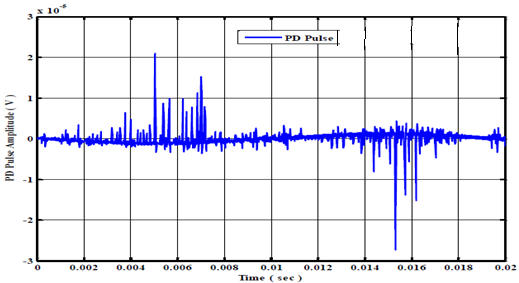
\includegraphics[width=\textwidth]{SineWaveofPartialDischarge}
    \caption{Sine Wave of Partial Discharge }
    \label{fig:Sine Wave of Partial Discharge }
\end{figure}
 
The Partial Discharge pulses are located with reference to the phase angle in positive and negative half cycle with respect to the phase angle.

The partial discharges due to the breakdown of insulation can be distinguished with the partial discharge with different types of discharges. The partial discharge pulses in the different quadrant can lead to a reoccurrence of discharges. With the voltage of 145 kV and different void sizes, the partial discharges pulse are shown in waveforms \cite{Dielectricwithstands}.

Results from the Simulink model has given various Partial discharge pulse, and it is observed that the density of PD is more at the center of positive and negative half cycle.Because of high insulation strength in high voltage Current Transformers, the breakdown in void will cause only when electric stress in the void excess strength of complete insulation. Therefore, PDs mostly appear at the center of half cycle of the sine waveform. 

\begin{figure}[h!]
    \centering
    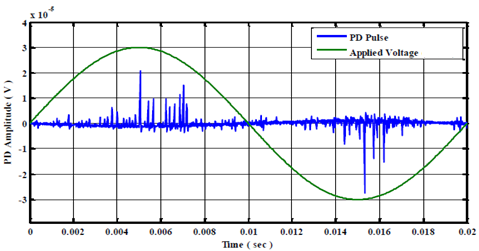
\includegraphics[width=\textwidth]{PartialDischargesinSinusoidalWaveform}
    \caption{Partial Discharges in Sinusoidal Waveform}
    \label{fig:Partial Discharges in Sinusoidal Waveform}
\end{figure}

From the partial discharge pulse for various void dimensions analysis has been done for the magnitude, density of pulse when 145 kV applied for different void sizes\setlength{\parskip}{0em}.

\clearpage
\subsubsection{Simulation waveforms of high voltage current transformers for different void dimensions during steady state conditions}

\begin{figure}[h!]
    \centering
    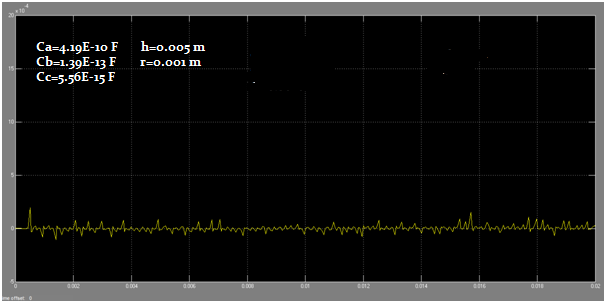
\includegraphics[width=\textwidth]{WaveformsforSteadyState1}\\
    \vspace{1cm}
    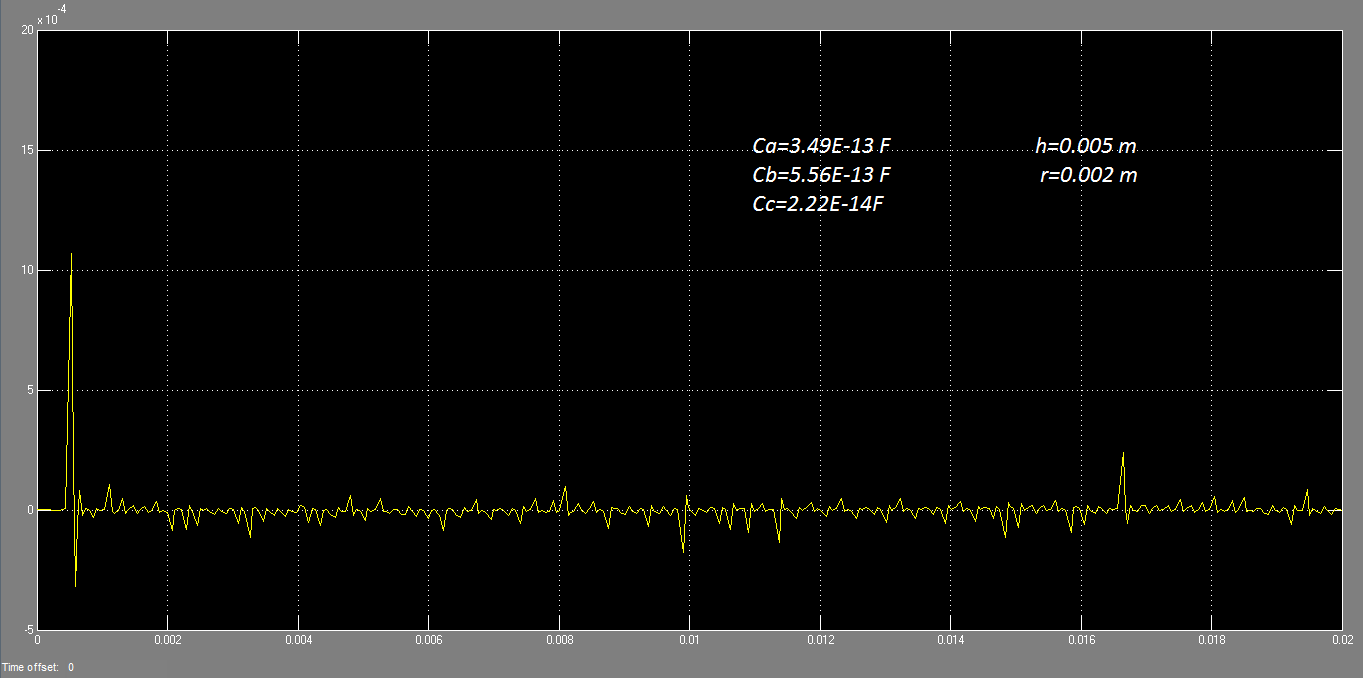
\includegraphics[width=\textwidth]{WaveformsforSteadyState2}
    \caption{Waveforms for Steady State}
    \label{fig:Waveforms for Steady State}
\end{figure}

The amplitude of the Pulse at the initial stage of the Positive waveform has increased as the dimensions of void increases.

\begin{center}
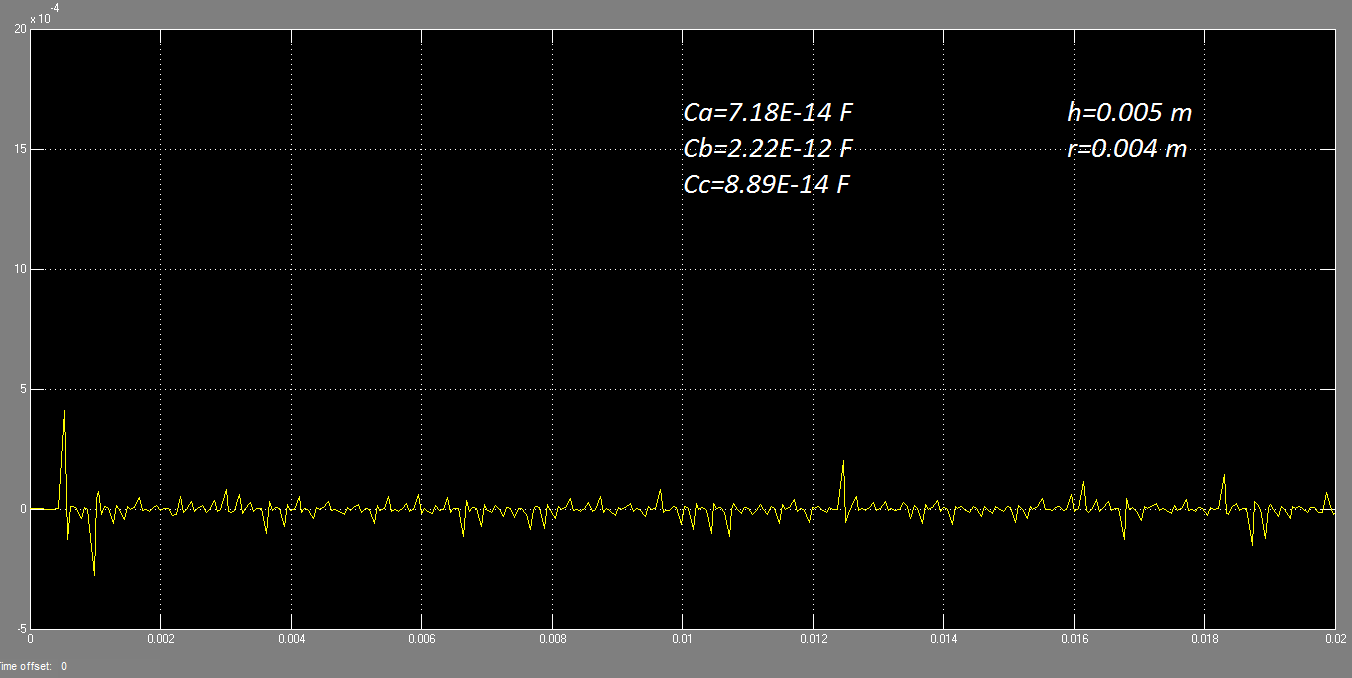
\includegraphics[width=\textwidth]{Wave3}
\vfill
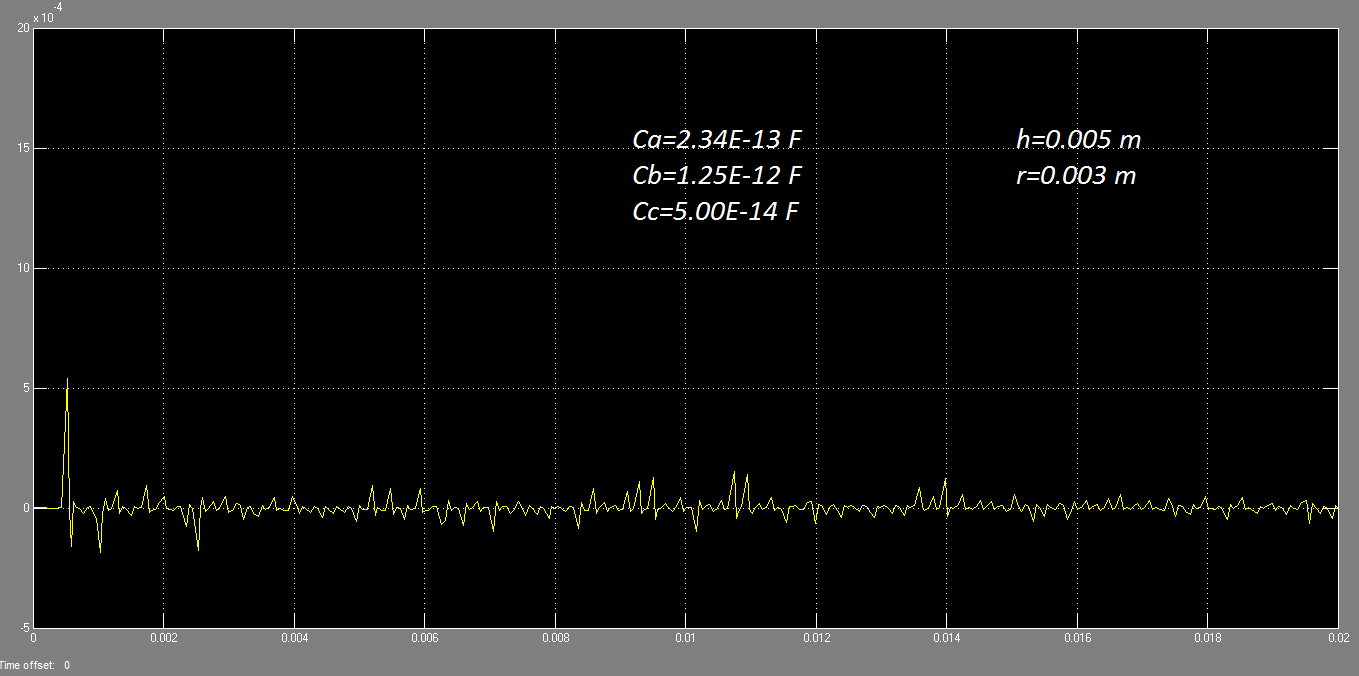
\includegraphics[width=\textwidth]{Wave4}
\vfill
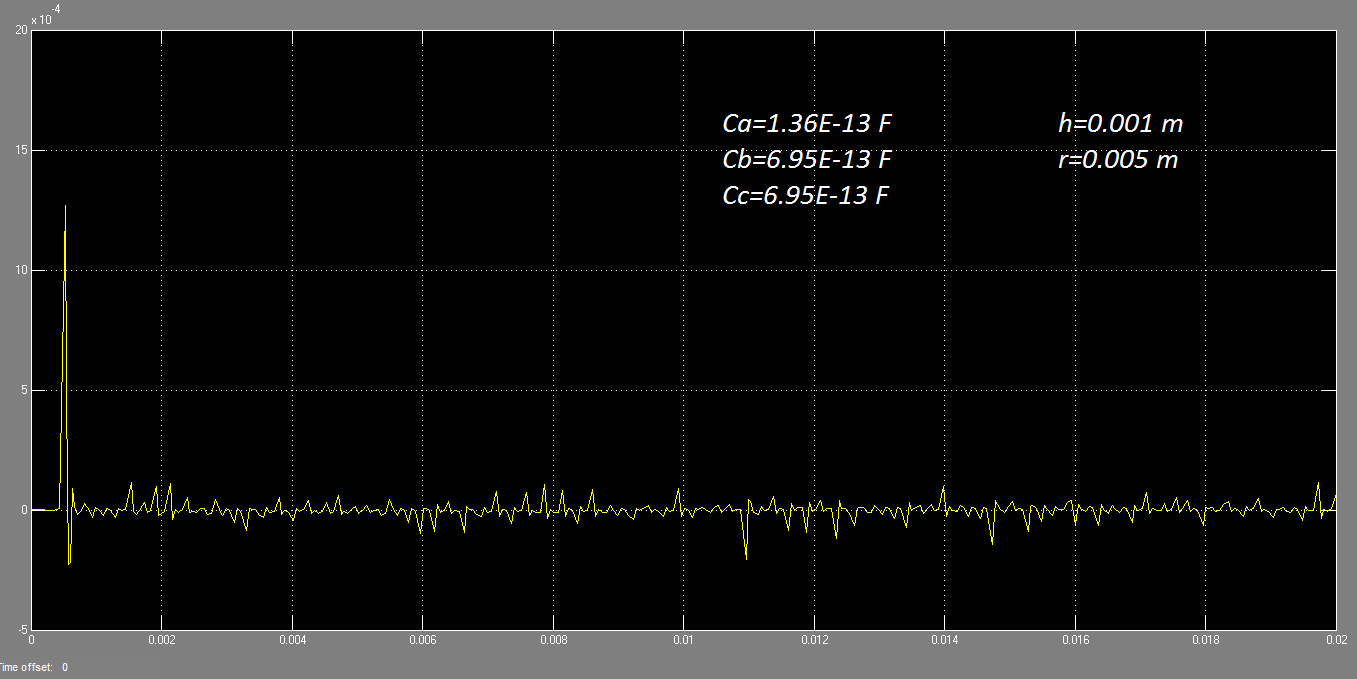
\includegraphics[width=\textwidth]{Wave5}
\end{center}
A number of PD Pulse Count is more in Negative Pulse.
The PD Level Waveform increases with increase in void dimensions.
\pagebreak

\begin{center}
\includegraphics[width=\textwidth]{Wave6}
\vfill
\includegraphics[width=\textwidth]{Wave7}
\vfill
\includegraphics[width=\textwidth]{Wave8}
\end{center}

\pagebreak
\begin{center}
\includegraphics[width=\textwidth]{Wave9}
\vfill
\includegraphics[width=\textwidth]{Wave91}
\vfill
\includegraphics[width=\textwidth]{Wave92}
\end{center}

\pagebreak
\begin{center}
\includegraphics[width=\textwidth]{Wave93}
\vfill
\includegraphics[width=\textwidth]{Wave94}
\vfill
\includegraphics[width=\textwidth]{Wave95}
\end{center}

The amplitude of the PD Pulse increases with increase in the waveform.

\pagebreak
\begin{center}
\includegraphics[width=\textwidth]{Wave96}
\vfill
\includegraphics[width=\textwidth]{Wave97}\\
Partial Discharge waveform is more in number as the dimensions of the void are more.
\vfill
\includegraphics[width=\textwidth]{Wave98}
\end{center}

\pagebreak
\begin{center}
\includegraphics[width=\textwidth]{Wave99}
\vfill
\includegraphics[width=\textwidth]{Wave991}
\vfill
\includegraphics[width=\textwidth]{Wave992}
\end{center}

\pagebreak
\begin{center}
\includegraphics[width=\textwidth]{Wave993}
\vfill
\includegraphics[width=\textwidth]{Wave994}
\vfill
\includegraphics[width=\textwidth]{Wave995}
\end{center}

\pagebreak
\begin{center}
\includegraphics[width=\textwidth]{Wave996}
\vfill
\includegraphics[width=\textwidth]{Wave997}
\vfill
\includegraphics[width=\textwidth]{Wave998}
\end{center}

\pagebreak
\begin{center}
\includegraphics[width=\textwidth]{Wave999}\\
Amplitude and frequency of PD waveform increase for higher void sizes. 
The Density of PD waveform, Pulses are more.
\vfill
\includegraphics[width=\textwidth]{Wave9991}
\vfill
\includegraphics[width=\textwidth]{Wave9992}
\end{center}

\pagebreak
\begin{center}
\includegraphics[width=\textwidth]{Wave9993}
\vfill
\includegraphics[width=\textwidth]{Wave9995}
\vfill
\includegraphics[width=\textwidth]{Wave9996}
\end{center}

\subsection[Analysis of simulation model for high voltage current transformers in short circuit and transient condition]{Analysis of simulation model for high voltage\\current transformers in short circuit and\\transient condition}

The performance of partial discharge was studied in short circuit and transient condition with Simulink model. The voltage of 145 kV was applied, and different void was provided in Simulink. The Capacitance values calculated as per the Table \ref{table:Values of Capacitance for Different Void Sizes} for $C_a$, $C_b$, $C_c$. System was run for the partial discharge pulses\setlength{\parskip}{1em}.

Enclosed ~all ~samples ~of ~partial ~discharge ~pulses ~waveform ~for ~different ~void conditions.

From the waveforms for different voids and calculated capacitance the magnitude of partial discharge changes with height, diameter and volume of the void. The capacitance changes with a change in dimensions of the void.

The capacitance values of different void sizes were calculated and shown in the table \ref{table:Values of Capacitance for Different Void Sizes}. The wave form for different capacitances is enclosed.

Conclusions from Simulation with Short Circuit and Transients Generated on Performance of Current Transformer

For various dimensions of voids and calculated capacitance $C_a$, $C_b$, $C_c$ Simulink model was run for short circuit and transient conditions on the system. The transients are a sudden short circuit in the line circuit. In this Simulink model, the magnetizing inductance and magnetizing current have been taken into account.

The Partial discharge activity inside the insulation of current transformer in a MATLAB Simulink model has taken for analysis and evaluation.

\begin{enumerate}
\item The Partial discharge activity inside the high voltage current transformers solid or oil insulation depends on the size of the void presence inside the oil and paper. The values of partial discharge increase with the voltage given to current transformer.

\item The PD waveform wave generated for different void were studied for magnitude, number, PD distribution and frequency of pulses.

\item In the Simulink model for Short circuit and Transient conditions, various capacitance values are put, and the system was run for the partial discharge waveform.

\item With change in Void parameters and voltage level Partial Discharge pulses varies, the density of PD's also varies

\item In ~high ~voltage ~current ~transformers ~the ~Partial ~Discharge ~can ~lead ~to deterioration of insulating material which can lead to the breakdown of live components in the long term.

\item The partial discharge process will change the properties of oil and other insulating media. With continuous discharge will leads to decomposition and pollution of the insulating oil as a result of which the insulation properties of the oil changes rapidly. 

\item Partial discharge measurement concludes the quality and strength of insulation inside the current transformers.

\item Specific phase related representation and assist and measure the identification of fault type 

\item PD pulse observed for 50 kV, 75 kV, 100 kV and 145 kV applied voltage between the test object has given different PD pulses for same void conditions\setlength{\parskip}{0em}.
\end{enumerate}
\pagebreak 

\subsubsection{Simulation waveforms of high voltage current transformers for different void dimensions during short circuit and transients}

\begin{figure}[h!]
    \centering
    \includegraphics[width=\textwidth]{WaveformsforTransient1}\\
    \vspace{1cm}
    \includegraphics[width=\textwidth]{WaveformsforTransient2}
    \caption{Waveforms for Transient}
    \label{fig:Waveforms for Transient}
\end{figure}

The effect of transients can be seen in the waveform as compared to steady state waveforms.

The frequency of PD waveforms are higher

Intermitted increase in the amplitude of waveform due to transients. 

\pagebreak
\begin{center}
\includegraphics[width=\textwidth]{TWave1}
\vfill
\includegraphics[width=\textwidth]{TWave2}
\vfill
\includegraphics[width=\textwidth]{TWave3}
\end{center}


\pagebreak
\begin{center}
As the dimensions of void increases, the magnitude of PD Pulses is more.
\includegraphics[width=\textwidth]{TWave4}
\vfill
\includegraphics[width=\textwidth]{TWave5}
\vfill
\includegraphics[width=\textwidth]{TWave6}
\end{center}

\pagebreak
\begin{center}
\includegraphics[width=\textwidth]{TWave7}
\vfill
\includegraphics[width=\textwidth]{TWave8}
\vfill
\includegraphics[width=\textwidth]{TWave9}
\vfill
A number of PD waveforms are more as the dimensions of the void are increased. 
\end{center}

\pagebreak
\begin{center}
\includegraphics[width=\textwidth]{TWaveA}
\vfill
\includegraphics[width=\textwidth]{TWaveB}
\vfill
\includegraphics[width=\textwidth]{TWaveC}
\end{center}

\pagebreak
\begin{center}
\includegraphics[width=\textwidth]{TWaveD}
\vfill
\includegraphics[width=\textwidth]{TWaveE}
\vfill
\includegraphics[width=\textwidth]{TWaveF}
\vfill
Distribution of PD Pulses is nonuniform for different void sizes.
\end{center}

\pagebreak
\begin{center}
\includegraphics[width=\textwidth]{TWaveG}
\vfill
\includegraphics[width=\textwidth]{TWaveH}
\vfill
\includegraphics[width=\textwidth]{TWaveI}
\end{center}

\pagebreak
\begin{center}
\includegraphics[width=\textwidth]{TWaveJ}
\vfill
\includegraphics[width=\textwidth]{TWaveK}
\vfill
\includegraphics[width=\textwidth]{TWaveL}
\end{center}

\pagebreak
\begin{center}
\includegraphics[width=\textwidth]{TWaveM}
\vfill
\includegraphics[width=\textwidth]{TWaveN}
\vfill
\includegraphics[width=\textwidth]{TWaveO}
\vfill
For particular dimensions of void, a linear variation observed in PD Pulses.
\end{center}

\pagebreak
\begin{center}
\includegraphics[width=\textwidth]{TWaveP}
\vfill
\includegraphics[width=\textwidth]{TWaveQ}
\vfill
\includegraphics[width=\textwidth]{TWaveR}
\end{center}

\pagebreak
\begin{center}
\includegraphics[width=\textwidth]{TWaveS}\\
\vspace*{1in}
\includegraphics[width=\textwidth]{TWaveT}
\end{center}

\pagebreak
\section{Analytical Analysis}
Based on the developed system discussed in chapter 3, a comprehensive analytical analysis is done for the following models considering the given mathematical equations and solving for steady state and short circuit and transient conditions\setlength{\parskip}{1em}.

\begin{enumerate}
\item Apparent charge 
\item Dimensions of voids
\item Accuracy of current transformers
\end{enumerate}

The dimensions of voids considered of various sizes from 0.001 m to 0.004 m as the volume of void increases, the capacitance increase, and the apparent charge increases. The effect on the phenomenon of partial discharge will lead to the formation of arcs . The deterioration of insulation takes place and can be evident from the partial discharge pulses.

\begin{enumerate}
\item Representation of voids in Capacitance 
\item Partial discharge pulse 
\end{enumerate}

The waveforms discussed in this chapter for during steady state conditions and transient conditions shows the intensity of partial discharge pulses. The intensity of pulse varies with the increase in capacitance of voids. The overall capacitance of void increases, the electrical stress in void increases due to this discharge increases to the extent of breakdown of the void \cite{bengtsson1997procedure}.

The waveforms due to transients show dense concentration of waves shows the partial discharge intensity. This intensity varies with the increase in capacitance, \textit{i.e.}, dimension of voids. These pulses were analyzed for void size varying from 0.001 m to 0.005 m. The amplitude, peak of the pulses, density of discharges can be evident to distinguish of pulse waveform for same voids in steady state operation of current transformers. 

The Capacitance values $C_a$, $C_b$, $C_c$ are calculated, and same values are used in Simulink Model for waveform pulses.

\begin{table}[h!]
\caption{Calculated Values of Capacitance 1}
\label{table:Calculated Values of Capacitance 1}
\centering
\begin{tabular}{|c|c|c|c|c|c|}
\hline 
Height of void 	&Radius of void &Sample dimension 				&$C_a$			&$C_b$			&$C_c$         \\ 
	(m)			&	(m) 		&								&(Farad) 		&(Farad) 		&(Farad)       \\ \hline \hline
0.005			&0.001			&.020$\times$.030$\times$.05 	&4.19$e^{-13}$	&1.39$e^{-13}$	&5.56$e^{-15}$ \\ \hline
0.005			&0.002			&.020$\times$.030$\times$.05 	&3.49$e^{-13}$	&5.56$e^{-13}$	&2.22$e^{-14}$ \\ \hline
0.005			&0.003			&.020$\times$.030$\times$.05 	&2.34$e^{-13}$	&1.25$e^{-12}$	&5.00$e^{-14}$ \\ \hline
0.005			&0.004			&.020$\times$.030$\times$.05 	&7.18$e^{-14}$	&2.22$e^{-12}$	&8.89$e^{-14}$ \\ \hline
0.005			&0.005			&.020$\times$.030$\times$.05 	&1.36$e^{-13}$	&3.47$e^{-12}$	&1.39$e^{-13}$ \\ \hline
\end{tabular} 
\end{table}

\begin{table}[h!]
\caption{Calculated Values of Capacitance 2}
\label{table:Calculated Values of Capacitance 2}
\centering
\begin{tabular}{|c|c|c|c|c|c|c|}
\hline 
Void & Void & Dimensions & \multicolumn{3}{c|}{Capacitance}  \\ 
\hline 
Geometry & Height & Radius &  All Insulation & Series with Void & Void \\  
• & m & m &  $C_a F$ & $C_b F$ & $C_c F$ \\ \hline \hline
\multirow{4}{*}{Ellipse}& 0.002	& 0.005	& 1.37$e^{-13}$	& 8.69$e^{-13}$	& 3.48$e^{-13}$ \\  \cline{2-6}
 		& 0.003	& 0.004	& 7.19$e^{-14}$	& 7.41$e^{-13}$	& 1.48$e^{-13}$ \\ \cline{2-6}
 		& 0.003	& 0.005	& 1.37$e^{-13}$	& 1.16$e^{-12}$	& 2.32$e^{-13}$ \\ \cline{2-6}
 		& 0.004	& 0.005	& 1.37$e^{-13}$	& 1.74$e^{-12}$	& 1.74$e^{-13}$ \\ \hline
\end{tabular} 
\end{table}

\begin{table}[h!]
\caption{Calculated Values of Capacitance 3}
\label{table:Calculated Values of Capacitance 3}
\centering
\begin{tabular}{|c|c|c|c|c|c|c|}
\hline 
Void & \multicolumn{3}{c|}{Void Dimensions} & \multicolumn{3}{c|}{Capacitance}  \\ 
\hline 
Geometry & Height & Radius & Area &  All Insulation & Series with Void & Void \\ 
• & m & m & m\textsuperscript{2} & $C_a F$ & $C_b F$ & $C_c F$ \\ \hline \hline 
			&0.005	&0.001	&0.0000032	&4.19$e^{-13}$	&1.39$e^{-13}$	&2.39$e^{-12}$ \\ \cline{2-7}
Irregular	&0.005	&0.002	&0.0000039	&3.50$e^{-13}$	&5.56$e^{-13}$	&9.62$e^{-12}$ \\ \cline{2-7}
 Shape		&0.005	&0.003	&0.0000045	&2.34$e^{-13}$	&1.25$e^{-12}$	&2.17$e^{-11}$ \\ \cline{2-7}
 			&0.005	&0.004	&0.0000055	&7.19$e^{-14}$	&2.22$e^{-12}$	&3.86$e^{-11}$ \\ \cline{2-7}
 			&0.005	&0.005	&0.0000032	&1.37$e^{-13}$	&3.48$e^{-12}$	&6.03$e^{-11}$ \\ \hline
\end{tabular} 
\end{table}

The capacitance values $C_a$, $C_b$, $C_c$ changes with void sizes. Capacitances values are calculated. Pulse waveforms for these waveforms show partial discharge phenomenon.

Relationship of Apparent charge to the size of the void is tabulated in the Table \ref{table:Apparent Charge with Different Void Sizes}. It shows the linear relationship.

\begin{table}[h!]
\caption{Apparent Charge with Different Void Sizes}
\label{table:Apparent Charge with Different Void Sizes}
\centering
\begin{tabular}{|c|c|c|c|c|}
\hline 
\multicolumn{3}{|c|}{Void Dimensions} &	Volume of Void	& Apparent Charge \\ \cline{1-3}
Height & Radius & Depth &  &  \\
m	&m	&m	& 	& 	\\ \hline \hline
0.005	&0.001	&0.001	&5$e^{-9}$&	2.00$e^{-14}$\\ \hline
0.005	&0.002	&0.001	&1$e^{-8}$&	3.88$e^{-14}$\\ \hline
0.005	&0.003	&0.001	&1.5$e^{-8}$&	5.67$e^{-14}$\\ \hline
0.005	&0.004	&0.001	&2$e^{-8}$&	7.98$e^{-14}$\\ \hline
0.005	&0.005	&0.001	&2.5$e^{-8}$&	9.83$e^{-14}$\\ \hline \hline
 	 	 	 	 
0.001	&0.001	&0.001	&1$e^{-9}$&	4.01$e^{-15}$\\ \hline
0.002	&0.002	&0.001	&4$e^{-9}$&	1.58$e^{-14}$\\ \hline
0.003	&0.003	&0.001	&9$e^{-9}$&	3.62$e^{-14}$\\ \hline
0.004	&0.004	&0.001	&1.6$e^{-8}$&	6.36$e^{-14}$\\ \hline
\end{tabular} 
\end{table}

Calculated values of Capacitance and waveforms from Simulink model shows the resemblance in the characteristics. 
\clearpage

\section[Comparison between Computational and Analytical Analysis]{Comparison between Computational and\\Analytical Analysis}
In all the models considered for the study during steady state and transients, the accuracy of current transformers changes considerably as the dielectric strength of insulating material changes which reflects in the performance and applications.

Enclosed readings of the accuracy of current transformers for various class. The accuracy performance of current transformers in steady state abruptly varies with the occurrence of transients.

\begin{table}[h!]
\caption{Accuracy Results of Different CT class}
\label{table:Accuracy Results of Different CT class}
\centering
\begin{tabular}{|c|c|c|c|c|}
\hline 
Sr. & CT Ratio Class	& Primary Current	& Steady state Ratio	& Transients Ratio \\
No. &					& \% 				& Error \% 				&  Error \% 		\\ \hline \hline
1	&0.5 S	& 		& 			& 			\\ \hline 
 	&3000/1 & 120	&	0.342	& 2.345 	\\ \hline 
 	&		& 100	&	0.331	& 2.456	\\ \hline 
 	&		& 20	& 0.129	& 1.341	\\ \hline 
 	&		& 5		& 0.012	&1.456	\\ \hline 
 	&		&120	&0.256	&2.023	\\ \hline 
 	&		&100	&0.237	&2.402	\\ \hline 
 	&		&20		&0.148	&1.890	\\ \hline 
 	&		&5		&0.126	&1.562	\\ \hline \hline
2	&PS		& 		& 			&			\\ \hline  
 	&2400/1	&100	&-0.034	&5.670	\\ \hline \hline
3	&5P		& 		& 			& 			\\ \hline 
 	&600/5	&100	&0.007	&3.15		\\ \hline \hline
4	&0.2 S	& 		& 			& 			\\ \hline 
 	&200/1	& 120	&0.116	&1.568	\\ \hline 
 	& 		& 100	&0.112	&1.558	\\ \hline 
 	& 		& 20	&0.076	&2.321	\\ \hline
 	&		& 5		&0.053	&2.291	\\ \hline
 	& 		& 120	&0.158	&1.628	\\ \hline
 	& 		& 100	&0.157	&1.601	\\ \hline
 	& 		& 20	&0.153	&1.289	\\ \hline
 	& 		& 5		&0.144	&1.243	\\ \hline
\end{tabular} 
\end{table}

The waveforms generated for various sizes of voids in the Simulink model in steady state and transients also shows the variations in partial discharge pulses resulting in the deterioration of the performance of current transformers. The amplitude, pulse, spike, density of partial discharge, frequency is shown in all waveforms are compared for the same void sizes in steady state and transient conditions. The distortion in the waveform is significant.

The results of performance distortion of oil filled current transformers 145 kV up to 3000 A by the computational method and analytical method shows same relevance in steady state and transient conditions due to the voids in insulating material or occurrence of partial discharge.  
\clearpage

\section{Justification for the difference}
The difference in the results obtained by the computational analysis and the analytical analysis discussed above is because one represents the performance regarding the numerical values and the other represents the performance in the wave form pulses. The computational analysis gives the distorted waveforms for the different values using the MATLAB/Simulink software is used for the simulation\setlength{\parskip}{0em}.

\chapter{CONCLUSIONS}
%Conclusion
\section{Conclusions}
\begin{itemize}
\item The Partial discharge inside the Current Transformer depends on the void present inside the oil and paper the magnitude and density of discharges is more during short circuit conditions 

\item The Partial discharge in current transformers increases with increase in magnitudes of voltage, deterioration of paper and oil insulation. The number of Partial Discharges, distribution, and magnitude of partial discharge, are sufficient to evaluate the performance of current transformers 

\item The magnitude, strength, and distribution of partial discharge pulses depend on the capacitance of voids. For same capacitance values in steady state condition and transient condition, partial discharge pulse will be different in magnitude and values 

\item Manufacturing Process needs to be carried out in controlled conditions with Low Vacuum Level less than o.5 mbar, Oil flow rate and temperature

\item The impact of PD in Steady State condition depends on relationship of Apparent Charge with Height, Volume, Radius of Voids

\item PD increases with magnitude and frequency of Short Circuit and Transients effect on Insulation
\end{itemize}
 
\pagebreak 

\section{Future Scope}
\begin{enumerate}
\item Effect of heat generated due to the transient on performance of Current Transformer 

\item Effect of switching ON/OFF circuit isolation of circuit Breaker on Current Transformer

\item Effect of super imposed voltage and current transient on source side and Load side
\end{enumerate}

\section{Applications}
From Simulink Model developed for study of Partial Discharge during Steady State, Short Circuit and Transient conditions Partial Discharge measurements can be done for Number of PD, Frequency of PD, Amplitude of PD for different Voltages up to 145 kV for various sizes of voids which will help in determining health and performance of High Voltage Current Transformers.

\clearpage
\section{Contributions}
\begin{itemize}
\item Analysis Model for High voltage oil filled current transformers 145 kV for comparison of waveforms in steady state and transients for different voids which give Amplitude, Frequency, Number of pulses of Partial Discharge

\item For different void sizes, partial discharge pulse was evolved for 145 kV Current Transformers during steady state and transients and are compared with to study effect on insulation strength of Oil and Papers

\item The results of performance distortion of oil filled current transformers 145 kV up to 3000 A by computational method and analytical method shows same relevance in steady state and transient conditions due to the voids in insulating material or occurrence of partial discharge
\end{itemize}
\clearpage

%\pagenumbering{gobble}
%\section*{Future Research Work}
%\begin{itemize}
%\item Effect of heat generated due to the transient on performance of Current Transformer
%
%\item Effect of switching ON/OFF ckt isolation of circuit Breaker on Current Transformer
%
%\item Effect of super imposed voltage and current transient on source side and Load side
%\end{itemize}
%\clearpage

%-------------------------References--------------------------------------------------------
\bibliographystyle{IEEEtran-mod}
\addcontentsline{toc}{chapter}{\numberline{}References}
\bibliography{References}
\clearpage

%-----------------------PUBLICATIONS---------------------------------------------------------
\section*{Publications}
\addcontentsline{toc}{chapter}{\numberline{}Publications}
\begin{enumerate}
\item \textquotedblleft ~Partial ~Discharge ~Analysis ~in ~High ~Voltage ~Current Transformers\textquotedblright, International Refereed Journal of Engineering and Sciences (IRJES), ISSN (Online) 2319-183X, Print 2319-1821, Vol. 6, Issue 5, May 2017, pp. 15-23.

\item \textquotedblleft Partial Discharge with Short Circuit and Transients Generated on Current Transformer\textquotedblright, 5th ~International ~Conference ~on ~Engineering ~Technology, Science and Management Innovation (ICETSMI-2017) at (IETE) Institution of Electronics and Telecommunication Engineers, 30th April 2017, ISBN: 978-81-933746-7-2, pp. 200-207.
\end{enumerate}
\clearpage

%-----------------------Appendix-----------------------------------------------------

\chapter*{Appendix}
\addcontentsline{toc}{chapter}{\numberline{}Appendix}
\setlength{\parskip}{1em}
\section*{Isolation Voltage}
The initial design of a device with an insulation barrier includes a choice of materials and dimensions to achieve an isolation voltage rating.

The isolation rating is the voltage level under specified conditions that the device will withstand without breakdown.

\section*{Isolation Voltage Failure Modes}
Isolation breakdown in devices can occur in several ways.

In an insulator, electrons are tightly bound to atoms and molecules. With moderate gradient ~potential, ~some ~electrons ~are ~pulled ~free ~of ~their ~bonds ~to be ~later recaptured in collisions with neighboring atoms or molecules. As the gradient is increased beyond the Intrinsic Dielectric Strength of the material, collisions occur with sufficient strength to free more electrons than are captured, resulting in a disruptive breakdown called Intrinsic Strength Breakdown. In another type of breakdown, a path across the surface of a device can lead to carbonization and possibly even Surface Flashover.

Another more complex cause of degradation failure inside the volume of the insulation material is Erosion Breakdown which will be later presented.

In High Voltage Leakage testing, the tester applies line frequency AC voltage and monitors the resulting device current to not exceed a certain limit. A good device will have both resistive and capacitive leakage components that are proportional to the instantaneous applied voltage. The resistive component of device impedance is typically in the order of Gigohms. A Leakage failure occurs when this resistance is degraded. Excessive device capacitance could also cause leakage failure, though a physical mechanism to cause this seems improbable.

\section*{Partial Discharge}
Partial discharges are the source of Erosion Breakdown which affects the long term life of an insulator. Partial discharges are discharges that do not completely bridge the insulation between the terminals. These discharges are termed “partial” because they occur in areas that occupy a small portion of the electrical path length and are limited in magnitude because they are in series with mostly good insulation (which may eventually degrade). These discharges can occur in insulators that contain gaseous inclusions, cavities, or voids.

\section*{Electric Field Basics--Electric Flux Density "D"}
Gauss’s Theorem states that the Electric Flux Density at a distance $r_1$ from a concentrated charge Q on a small conductive sphere may be determined by enlarging the sphere until its radius is equal to $r_2$ (as the charge is distributed in equilibrium on the surface). The magnitude of the Electric Flux Density at $r_2$ is the charge Q divided by the surface area of the enlarged sphere.

\section*{Electric Field Intensity}
The strength and direction of the Electric Field Intensity of any point in an electric field may be measured by the force and direction upon a test charge. Electric Field Intensity measured in Newtons per Coulomb (dimensionally equivalent to Volts per meter) may be thought of as the force effectiveness of the electric field.

\section*{Medium Relative Permittivity (e\textsubscript{r})}
\begin{tabular}{l l}
Vacuum	& 1 \\
Air	& 1.006\\
Styrofoam	& 1.03\\
Polystyrene	& 2.7\\
Plexiglass	& 3.4\\
Amber	& 3\\
Rubber &3 \\
\end{tabular}

\section*{Rated voltage}
The rated voltage is the maximum voltage (phase-phase), expressed in kV rms, of the system for which the equipment is intended. It is also known as maximum system voltage.

\section*{Rated insulation level}
The combination of voltage values which characterize the insulation of an instrument transformer with regard to its capability to withstand dielectric stresses.
\section*{Lightning impulse test}
The lightning impulse test is performed with a standardized wave shape – 1.2/50 $\mu s$ – for simulation of lightning overvoltage.
\section*{Rated Power Frequency Withstand Voltage}
This test is to show that the apparatus can withstand the power frequency over-voltages that can occur.

The Rated Power Frequency Withstand voltage indicates the required withstand voltage. The value is expressed in kV rms.

\section*{Rated SIWL}
For voltages ≥300 kV the power-frequency voltage test is partly replaced by the switching impulse test. The wave shape 250/2500 μs simulates switching over-voltage. The rated Switching Impulse Withstand Level (SIWL) indicates the required withstand level phase-to-earth (phase to- ground), between phases and across open contacts. The value is expressed in kV as a peak value.
\section*{Rated Chopped Wave Impulse Withstand voltage, Phase-to-earth}
The rated chopped wave impulse withstand level at 2 $\mu s$ and 3 $\mu s$ respectively, indicates the required withstand level phase-to-earth (phase-to-ground).

\section*{Rated frequency}
The rated (power) frequency is the nominal frequency of the system expressed in Hz, which the instrument transformer is designed to operate in Standard frequencies are 50 Hz 

\section*{Ambient temperature}
Average 24 hours ambient temperature above the standardized +35 \textdegree C influences the thermal design of the transformers and must, therefore, be specified.

\section*{Creepage distance}
The creepage distance is defined as the shortest distance along the surface of an insulator between high voltage and ground. The rated currents are the values of primary and secondary currents on which performance is based. 

\section*{Rated primary current}
The rated current (sometimes referred to as rated current, nominal current or rated continuous current) is the maximum continuous current the equipment is allowed to carry. The current is expressed in an rms. The maximum continuous thermal current is based on average 24 h ambient temperature of +35 \textdegree C. It should be selected about 10 - 40\% higher than the estimated operating current. The closest standardized value should be chosen.

\section*{Extended current ratings}
A factor that multiplied by the rated current gives the maximum continuous load current and the limit for accuracy. Standard values of extended primary current are 120, 150 and 200\% of rated current. Unless otherwise specified, the rated continuous thermal current shall be the rated primary current.
\section*{Rated secondary current}
The standard values are 1, 2 and 5 A. 1 A gives an overall lower burden requirement through lower cable burden.
\section*{Rated short-time thermal current (I\textsubscript{th})}
The rated short-time withstand current is the maximum current (expressed in kA rms) which the equipment shall be able to carry for a specified time duration. Standard values for duration are 1 or 3 s. $I_th$ depends on the short-circuit power of the grid and can be calculated from the formula:
\[
I_{th} = Pk (MW) / Um (kV) \times \sqrt{3} kA.
\]
\section*{Rated dynamic current (I\textsubscript{dyn})}
The dynamic short-time current is according to IEC, $I_{dyn} = 2.5 \times I_{th}$ and according to IEEE, $I_{dyn} = 2.7 \times I_{th}$

\section*{Reconnection}
Current transformer can be designed with either primary or secondary reconnection or a combination of both to obtain more current ratios.
\section*{Primary reconnection}
The ampere-turns always remain the same and thereby the load capacity (burden) remains the same. The short-circuit capacity, however, may be reduced for the lower ratios. Primary reconnection is available for currents in relation 2:1 or 4:2:1.
\section*{Secondary reconnection}
Extra secondary terminals (taps) are taken out from the secondary winding. The load capacity drops as the ampere-turns decrease on the taps, but the short-circuit capacity remains constant. Each core can be individually reconnected.
\section*{Burden}
The external impedance in the secondary circuit in ohms at the specified power factor. It is usually expressed as the apparent power in VA, which is taken up at rated secondary current. It is important to determine the power consumption of connected meters and relays including the cables. Unnecessarily high burdens are often specified for modern equipment. Note that the accuracy for the measuring core, according to IEC, can be outside the class limit if the actual burden is below 25\% of the rated burden.

\section*{Accuracy}
The accuracy class for measuring cores is according to the IEC standard given as 0.2, 0.2S, 0.5, 0.5S or 1.0 depending on the application. For protection cores, the class is normally 5P or 10P. Other classes are quoted on request, e.g., class PR, PX, TPS, TPX or TPY.
\section*{Resistance}
The secondary winding resistance at 75 \textdegree C
\section*{Instrument Security Factor (IFS)}
To protect meters and instruments from being damaged by high currents, an FS factor of 5 or 10 is often specified for measuring cores. This means that the secondary current will increase maximum 5 or 10 times when the rated burden is connected. FS10 is normally sufficient for modern meters.
\section*{Accuracy Limit Factor (ALF)}
The protection cores must be able to reproduce the fault current without being saturated. The over current factor for protection cores is called ALF. ALF = 10 or 20 is commonly used. Both FS and ALF are valid at rated burden only. If lower burden the FS and ALF will increase.
\setlength{\parskip}{0em}
\clearpage

%-----------------------ACKNOWLEDGEMENT------------------------------------------------------

\begin{center}
\large \textbf{ACKNOWLEDGEMENT}
\addcontentsline{toc}{chapter}{\numberline{}Acknowledgement}
\end{center}

\setlength{\parskip}{1em}
\justify \normalsize I, take this opportunity to thank my guide \textbf{Dr. W. Z. Gandhare, Director, G. S. Moze College of Engineering, Pune} for his intense valuable guidance and constant motivation during the entire research work.

I wish to thank Internal Monitoring Committee Members \textbf{Dr. M. G. Shaikh, Dr. Mrs. A. S. Bhalchandra, Dr. R. V. Shetkar} and \textbf{Dr. A. G. Thosar}, Head of Electrical Engineering Department, Government College of Engineering, Aurangabad for their valuable support, suggestions and extending all the facilities for completion of this research work. I would like to appreciate the support and help given by my colleagues and all staff members of the institute.

I am thankful to \textbf{Dr. P. V. Murnal}, Principal, Government College of Engineering, Aurangabad for his valuable suggestions which helped me to accomplish this task. 

Finally, I would like to thank my brothers \textbf{Dr. Deepak, Mrs. Nilima} and \textbf{Dr. Vivek, Mrs. Jayeshsree} for their inspiration from childhood to till this study, wife \textbf{Mrs. Anupama}, children \textbf{Veena} and \textbf{Vaibhav} for their help and consistent encouragement without which it could not be possible for me to complete the research work.


\setlength{\parskip}{0em}
\vspace{2cm}
\begin{flushright}
\textbf{Vinayak Shankarrao Deolankar}
\end{flushright}

%\printindex

\end{document}